\chapter{連通性：強連通元件、割點、橋與雙連通元件}
\label{ch:connectivity}

% 本章的圖共用的樣式（前綴 con-）。 追蹤表和圖上的 d、f、low 都由模擬程式照虛擬碼
% 逐步執行後產生，再和本章的 C 程式輸出對過。
\tikzset{
    con-v/.style={circle, draw=black!70, fill=white, minimum size=0.62cm, inner sep=0pt, font=\small},
    con-cut/.style={draw=memStroke, very thick, fill=memFill},
    con-arc/.style={-{Stealth[length=1.8mm]}, draw=black!60, shorten >=0.5pt},
    con-tree/.style={draw=black, very thick},
    con-nt/.style={densely dashed},
    con-elab/.style={font=\scriptsize, fill=white, inner sep=0.8pt, text=black!75},
    con-lab/.style={font=\scriptsize, text=black!80},
    con-scc/.style={rounded corners=7pt, fill=coreFill, draw=coreStroke!50, inner sep=5pt},
    con-sccname/.style={font=\scriptsize, text=coreStroke},
    con-cv/.style={rounded corners=3pt, draw=coreStroke!70, fill=coreFill, font=\small, inner sep=4pt},
    con-e/.style={draw=black!60, thick},
    con-bridge/.style={draw=optStroke, line width=1.8pt},
    con-back/.style={draw=black!55, densely dashed, thick},
}

市政府把老城區的十幾條路改成單行道。 改完以後，交通局想先確認兩件事：從任何一個路
口出發，是不是都還能開到其他路口；如果不能，哪些路口之間可以來回，哪些只能單向進
出。 另一邊，學校要整修校園裡的大樓和走廊，一次只封一棟或一條。 總務處想知道，封
掉哪一棟大樓、哪一條走廊，會讓其他大樓之間走不通。 這兩個問題都可以一個一個試：每
封一處就從頭走一遍圖，看還連不連通。 往下讀之前，先想想有沒有辦法只走一遍圖，就把
答案全部找出來。

這一章用第~21~章的深度優先搜尋（DFS）回答這兩類問題。 有向圖的部分是\textbf{強連
通元件}：把「彼此可以來回」的頂點分成一群一群。 我們會講兩個 $\Theta(n + m)$ 的演
算法：Kosaraju 演算法做兩次 DFS，第二次在把邊全部反向的圖上做；Tarjan 演算法只做
一次 DFS，用一個叫 $\mathit{low}$ 的值和一個堆疊。 每一群縮成一個點以後，得到的圖一定
沒有環，第~22~章的拓樸排序就能用上。 無向圖的部分是\textbf{割點}、\textbf{橋}和
\textbf{雙連通元件}，也用 $\mathit{low}$ 值判斷，寫法和 Tarjan 演算法很像，但細節不
同，考試最常考的就是這張 $\mathit{low}$ 值的手算表。

這一章用到第~21~章的這些東西：鄰接串列、DFS 的白灰黑三色和時間戳記 $d[v]$、$f[v]$、
DFS 森林、括號定理（定理~\ref{thm:gtr-paren}）、白路徑定理（定理~\ref{thm:gtr-whitepath}），以及有向圖的四種邊（樹邊、後向邊、前向邊、交叉
邊）。 第~22~章「依完成時間由大到小排列」的拓樸排序法也會用到。 程式方面用到《C 程
式設計基礎》第~14~章的結構、第~15~章的遞迴和第~19~章的 \texttt{malloc}、鏈結串
列。

本章的約定和第~21~章相同：圖有 $n$ 個頂點、$m$ 條邊，頂點編號 $1$ 到 $n$（觀念題有
時用英文字母）；鄰接串列裡每個頂點的鄰居由小到大排，DFS 照這個順序走，主迴圈也從
編號小的頂點開始。 C 程式裡的頂點從 $0$ 編號，讀入時減一、印出時加一，所以輸出和手
算用的是同一套編號。

\section{強連通元件}
\label{sec:con-scc}

記號照第~21~章：有向圖裡有一條從 $u$ 到 $v$ 的路徑，就說 $v$ 可以從 $u$ 到達，記成
$u \leadsto v$。 長度 $0$ 的路徑也算，所以每個頂點都可以到達自己。 第~21~章已經簡單介紹過強連
通元件，這裡寫成正式的定義。

\begin{definition}
有向圖 $G = (V, E)$ 裡，如果 $u \leadsto v$ 而且 $v \leadsto u$，就說 $u$ 和 $v$
\textbf{互相可達}。 \textbf{強連通元件}（strongly connected component，簡稱 SCC）是
一個最大的頂點集合 $C \subseteq V$，其中任兩個頂點都互相可達。「最大」的意思是再
加進任何一個 $C$ 以外的頂點，這個性質就不成立。 整張圖只有一個強連通元件時，叫做
\textbf{強連通}（strongly connected）的圖。
\end{definition}

「互相可達」是一個\textbf{等價關係}：每個頂點和自己互相可達（長度 $0$ 的路徑）；
$u$、$v$ 互相可達時 $v$、$u$ 也是；$u$、$v$ 互相可達、$v$、$w$ 互相可達，把路徑接起
來就得到 $u$、$w$ 互相可達。 等價關係把頂點分成互不重疊的類別，每一類就是一個強連通
元件。 所以每個頂點恰好屬於一個強連通元件，元件可以只有一個頂點。

\begin{center}
\begin{tikzpicture}[x=1.15cm, y=1.15cm]
\node[con-v] (v1) at (1.5,1.8) {1};
\node[con-v] (v2) at (3.3,1.8) {2};
\node[con-v] (v3) at (2.6,-0.9) {3};
\node[con-v] (v4) at (2.4,0.45) {4};
\node[con-v] (v5) at (5.1,-0.3) {5};
\node[con-v] (v6) at (5.1,1.8) {6};
\node[con-v] (v7) at (0,0.9) {7};
\node[con-v] (v8) at (0.9,-0.9) {8};
\node[con-v] (v9) at (6.5,0.75) {9};
\begin{scope}[on background layer]
\node[con-scc, fit=(v1)(v2)(v4)] (s2) {};
\node[con-scc, fit=(v3)(v8)] (s3) {};
\node[con-scc, fit=(v5)(v6)(v9)] (s4) {};
\node[con-scc, fit=(v7)] (s1) {};
\end{scope}
\node[con-sccname, anchor=south] at (s1.north) {$C_1$};
\node[con-sccname, anchor=south] at (s2.north) {$C_2$};
\node[con-sccname, anchor=north] at (s3.south) {$C_3$};
\node[con-sccname, anchor=south] at (s4.north) {$C_4$};
\draw[con-arc] (v1) to[bend left=14] (v2);
\draw[con-arc] (v2) to[bend left=14] (v1);
\draw[con-arc] (v1) -- (v4);
\draw[con-arc] (v2) -- (v6);
\draw[con-arc] (v3) -- (v5);
\draw[con-arc] (v3) to[bend left=14] (v8);
\draw[con-arc] (v8) to[bend left=14] (v3);
\draw[con-arc] (v4) -- (v2);
\draw[con-arc] (v4) -- (v3);
\draw[con-arc] (v5) -- (v6);
\draw[con-arc] (v6) -- (v9);
\draw[con-arc] (v9) -- (v5);
\draw[con-arc] (v7) -- (v1);
\draw[con-arc] (v7) -- (v8);
\end{tikzpicture}
\diagcaption{老城區的單行道路網：$9$ 個路口、$14$ 條單行道。 藍底的四塊是四個強連通
元件 $C_1 = \{7\}$、$C_2 = \{1, 2, 4\}$、$C_3 = \{3, 8\}$、$C_4 = \{5, 6, 9\}$。}
\label{fig:con-roads}
\end{center}

圖~\ref{fig:con-roads} 是章首的路網，本章前四節都用它。 $1 \to 4 \to 2 \to 1$ 是一
個環，所以 $1, 2, 4$ 互相可達；$3$ 和 $8$ 之間兩個方向都有路；$6 \to 9 \to 5 \to 6$
又是一個環。 路口 $7$ 沒有任何路開進來，除了自己以外沒有誰能到 $7$，所以它自己一個元
件。 元件之間的路都只有一個方向：從 $C_2$ 可以經過 $2 \to 6$ 進入 $C_4$，但 $C_4$
裡沒有任何一條路開出去，一開進 $C_4$ 就回不到其他元件。

\subsection{轉置圖和元件圖}

把 $G$ 的每一條邊都反向，得到\textbf{轉置圖} $G^{\mathrm{T}} = (V, E^{\mathrm{T}})$，
其中 $E^{\mathrm{T}} = \{(v, u) : (u, v) \in E\}$。 $G$ 裡從 $u$ 到 $v$ 的路徑反過來，
就是 $G^{\mathrm{T}}$ 裡從 $v$ 到 $u$ 的路徑，所以「互相可達」在兩張圖裡完全一樣：
\textbf{$G$ 和 $G^{\mathrm{T}}$ 的強連通元件相同}。 用鄰接串列表示時，掃一遍所有的
邊、把每條 $(u, v)$ 加進 $G^{\mathrm{T}}$ 的 $v$ 的串列，花 $\Theta(n + m)$ 時間。

把每個強連通元件縮成一個點，得到的圖叫\textbf{元件圖}（component graph），記成
$G^{\mathrm{SCC}}$：它的頂點是 $G$ 的強連通元件 $C_1, C_2, \ldots, C_k$；只要 $G$ 裡
有一條邊從 $C_i$ 的某個頂點指到 $C_j$ 的某個頂點（$i \ne j$），就加一條邊 $(C_i,
C_j)$，同一對元件之間最多一條。 元件內部的邊縮掉了，不留自環。

\begin{lemma}
\label{lem:con-dag}
任何有向圖的元件圖都沒有環，也就是說 $G^{\mathrm{SCC}}$ 是一個 DAG。
\end{lemma}

\begin{proof}
假設元件圖有一個環 $C_1 \to C_2 \to \cdots \to C_j \to C_1$，$j \ge 2$，而且這些元
件互不相同。 邊 $(C_i, C_{i+1})$ 表示有 $x \in C_i$、$y \in C_{i+1}$ 使得 $(x, y)
\in E$。 元件裡的頂點互相可達，所以 $C_i$ 的任何頂點都能先走到 $x$，經過 $(x, y)$，
再走到 $C_{i+1}$ 的任何頂點。 沿著環走一圈，$C_1$ 的頂點能到 $C_2$ 的頂點，$C_2$ 的頂點
也能繞回 $C_1$ 的頂點，兩者互相可達，應該在同一個元件裡，和 $C_1 \ne C_2$ 矛盾。
\end{proof}

最直接的找法是從每個頂點各做一次 DFS，求出它能到哪些頂點，再把互相可達的配對起
來。 這要做 $n$ 次 DFS，總共 $O(n(n + m))$。 接下來兩節的演算法都只要 $\Theta(n + m)$。

\section{Kosaraju 演算法}
\label{sec:con-kosaraju}

先想一個比較容易的情況。 假設我們知道某個元件 $C$ 在元件圖裡是\textbf{匯點}（沒有
邊出去），從 $C$ 裡的任何一個頂點開始做 DFS，走得到的頂點都在 $C$ 裡，而且 $C$ 的每
個頂點都走得到，這一棵 DFS 樹剛好就是 $C$。 把 $C$ 拿掉以後，剩下的元件圖還是 DAG，
一定還有匯點，再從那裡做一次……每次都從匯點開始，就能把元件一個一個剝下來。

問題是我們不知道匯點在哪裡。 Kosaraju 演算法的想法是：先對 $G$ 做一次完整的 DFS，
\textbf{完成時間最大的頂點一定落在元件圖的源點}（沒有邊進來的元件）。 $G$ 的源點元件
在 $G^{\mathrm{T}}$ 裡正好變成匯點元件，所以第二次 DFS 改在 $G^{\mathrm{T}}$ 上做，
依完成時間由大到小挑起點，每一棵樹就是一個強連通元件。

\begin{pseudo}[label=alg:con-kosaraju]{Kosaraju 演算法}
\Procedure{Kosaraju}{$G$}
    \State 對 $G$ 做第~21~章的 DFS，求出每個頂點的完成時間 $f[u]$
    \State 建立轉置圖 $G^{\mathrm{T}}$
    \State 把每個 $\mathit{comp}[u]$ 設成 $0$；$k \gets 0$
    \For{依 $f[u]$ 由大到小的每個頂點 $u$}
        \If{$\mathit{comp}[u] = 0$}
            \State $k \gets k + 1$
            \State \Call{Assign}{$G^{\mathrm{T}}, u, k$}
        \EndIf
    \EndFor
\EndProcedure
\Procedure{Assign}{$H, u, k$}
    \State $\mathit{comp}[u] \gets k$ \Comment{$u$ 屬於第 $k$ 個元件}
    \For{每個 $v \in H.\mathit{Adj}[u]$}
        \If{$\mathit{comp}[v] = 0$}
            \State \Call{Assign}{$H, v, k$}
        \EndIf
    \EndFor
\EndProcedure
\end{pseudo}

第 5 行要的「依 $f$ 由大到小」的順序不用另外排序：和第~22~章的拓樸排序一樣，每個
頂點在第 2 行的 DFS 完成時就把它插到一個串列的最前面，DFS 做完時，串列就是完成時間由大到小
的順序。 \proc{Assign} 是只做「發現」的 DFS，用 $\mathit{comp}[v] = 0$ 代表白色。 兩
次 DFS 和建立 $G^{\mathrm{T}}$ 各花 $\Theta(n + m)$，總時間是 $\Theta(n + m)$。

\subsection{為什麼對}

下面的 $d[u]$、$f[u]$ 都指第一次 DFS（在 $G$ 上）的時間戳記。 對一個頂點集合 $C$，令
$f(C) = \max\{f[u] : u \in C\}$，也就是 $C$ 裡最晚完成的時間。

\begin{lemma}
\label{lem:con-finish}
設 $C$、$C'$ 是 $G$ 的兩個不同的強連通元件，而且有一條邊 $(x, y) \in E$，$x \in C$、
$y \in C'$。 那麼 $f(C) > f(C')$。
\end{lemma}

\begin{proof}
令 $z$ 是 $C \cup C'$ 裡最先被發現的頂點。 在時間 $d[z]$，$C \cup C'$ 的頂點全是白
色。 分兩種情況。

\textbf{$z \in C$}。 $C$ 裡任何頂點都能從 $z$ 在 $C$ 裡面走到；$C'$ 的任何頂點 $v$
也能從 $z$ 走到：先在 $C$ 裡走到 $x$，經過 $(x, y)$，再在 $C'$ 裡走到 $v$。 這些路徑
只經過 $C \cup C'$ 的頂點，在時間 $d[z]$ 全是白色，由白路徑定理，$C \cup C'$ 的其他
頂點都是 $z$ 在 DFS 樹裡的子孫。 由括號定理，子孫比 $z$ 先完成，所以 $f(C) = f[z] >
f(C')$。

\textbf{$z \in C'$}。 同樣的理由，$C'$ 的其他頂點都是 $z$ 的子孫，$f(C') = f[z]$。
$z$ 走不到 $C$ 的任何頂點：如果走得到，加上邊 $(x, y)$ 和 $C'$ 內部的路，$C$ 和 $C'$
就互相可達了。 在 $d[z]$ 到 $f[z]$ 這段時間裡被發現的頂點都是 $z$ 的子孫（括號定理），
也都從 $z$ 走得到，所以 $C$ 的頂點在時間 $f[z]$ 仍然是白色，之後才被發現、完成。 因此
$C$ 的每個頂點的完成時間都大於 $f[z]$，$f(C) > f[z] = f(C')$。
\end{proof}

換句話說，元件圖裡每一條邊 $(C, C')$ 都從 $f$ 較大的元件指向 $f$ 較小的元件。 完成時
間最大的頂點所在的元件 $f$ 值最大，不可能有邊指進來，是一個源點。

\begin{theorem}
\label{thm:con-kosaraju}
虛擬碼~\ref{alg:con-kosaraju} 第二次 DFS 的每一棵樹（同一個 $k$ 的頂點）恰好是一個強
連通元件。
\end{theorem}

\begin{proof}
對樹的個數做歸納。 假設前 $k - 1$ 棵樹各是一個完整的強連通元件，看第 $k$ 棵樹，它的
根 $r$ 是目前 $\mathit{comp} = 0$ 的頂點裡 $f$ 最大的一個。 令 $C$ 是 $r$ 所在的元件。
由歸納假設，已經分好的頂點都屬於完整的元件，$C$ 不是其中之一，所以 $C$ 的頂點全都還
沒分。 於是 $f[r] = f(C)$，而且對每個還沒分的元件 $C''$ 都有 $f(C) \ge f(C'')$。

(1) $C$ 的頂點都在這棵樹裡。 $C$ 在 $G^{\mathrm{T}}$ 裡也是強連通的，開始 $\proc{Assign}
(G^{\mathrm{T}}, r, k)$ 時 $C$ 的頂點全是白色（$\mathit{comp} = 0$），由白路徑定理，它
們都會成為 $r$ 的子孫。

(2) 這棵樹沒有 $C$ 以外的頂點。 假設有，看第一個被加進來、不在 $C$ 裡的頂點 $v$：它
是從樹裡某個頂點 $u$ 沿著 $G^{\mathrm{T}}$ 的邊 $(u, v)$ 走到的，而 $u$ 在 $C$ 裡。
$G^{\mathrm{T}}$ 的邊 $(u, v)$ 就是 $G$ 的邊 $(v, u)$，從 $v$ 的元件 $C_v$ 指向 $C$，
由引理~\ref{lem:con-finish}，$f(C_v) > f(C)$。 但 $v$ 的 $\mathit{comp}$ 是 $0$，
$C_v$ 還沒分，這和 $f(C)$ 是還沒分的元件裡最大的矛盾。
\end{proof}

證明的 (2) 也說明了第二次 DFS 為什麼一定要在 $G^{\mathrm{T}}$ 上做。 如果還在 $G$
上，從源點元件出發會順著邊走進下游的元件，一棵樹就吃下好幾個元件。

再看元件產生的順序。 第 $k$ 棵樹的根是當時 $f$ 最大的頂點，所以 $f(C_1) > f(C_2) >
\cdots$。 由引理~\ref{lem:con-finish}，元件圖的邊 $(C_i, C_j)$ 一定滿足 $f(C_i) >
f(C_j)$，也就是 $i < j$。 所以 \textbf{Kosaraju 演算法依元件圖的拓樸順序產生元件}，
第~\ref{sec:con-dag}~節會用到這一點。

\subsection{手算追蹤}

在圖~\ref{fig:con-roads} 的路網上跑一次。 第一次 DFS 在 $G$ 上，從 $1$ 開始，鄰居由小到大：
$1 \to 2$，$2$ 的鄰居 $1$ 是灰色（後向邊），接著 $2 \to 6 \to 9 \to 5$；$5 \to 6$ 是
後向邊，$5$、$9$、$6$、$2$ 依序完成。 回到 $1$，走 $1 \to 4$：$4 \to 2$ 時 $2$ 已經是
黑色，而且 $d[2] < d[4]$，是交叉邊；$4 \to 3$，$3 \to 5$ 又是交叉邊，$3 \to 8$，$8
\to 3$ 是後向邊。 最後主迴圈走到 $7$，它的兩條邊都指向黑色的頂點，是交叉邊。

\begin{center}
\begin{tikzpicture}[x=1.15cm, y=1.15cm]
\node[con-v] (v1) at (1.5,1.8) {1};
\node[con-v] (v2) at (3.3,1.8) {2};
\node[con-v] (v3) at (2.6,-0.9) {3};
\node[con-v] (v4) at (2.4,0.45) {4};
\node[con-v] (v5) at (5.1,-0.3) {5};
\node[con-v] (v6) at (5.1,1.8) {6};
\node[con-v] (v7) at (0,0.9) {7};
\node[con-v] (v8) at (0.9,-0.9) {8};
\node[con-v] (v9) at (6.5,0.75) {9};
\node[con-lab, above=0.5mm of v1] {1/16};
\node[con-lab, above=0.5mm of v2] {2/9};
\node[con-lab, below=0.5mm of v3] {11/14};
\node[con-lab, right=0.5mm of v4] {10/15};
\node[con-lab, below=0.5mm of v5] {5/6};
\node[con-lab, above=0.5mm of v6] {3/8};
\node[con-lab, above=0.5mm of v7] {17/18};
\node[con-lab, below=0.5mm of v8] {12/13};
\node[con-lab, right=0.5mm of v9] {4/7};
\draw[con-arc, con-tree] (v1) to[bend left=14] (v2);
\draw[con-arc, con-nt] (v2) to[bend left=14] node[con-elab, below] {B} (v1);
\draw[con-arc, con-tree] (v1) -- (v4);
\draw[con-arc, con-tree] (v2) -- (v6);
\draw[con-arc, con-nt] (v3) -- node[con-elab, pos=0.55] {C} (v5);
\draw[con-arc, con-tree] (v3) to[bend left=14] (v8);
\draw[con-arc, con-nt] (v8) to[bend left=14] node[con-elab, above] {B} (v3);
\draw[con-arc, con-nt] (v4) -- node[con-elab] {C} (v2);
\draw[con-arc, con-tree] (v4) -- (v3);
\draw[con-arc, con-nt] (v5) -- node[con-elab] {B} (v6);
\draw[con-arc, con-tree] (v6) -- (v9);
\draw[con-arc, con-tree] (v9) -- (v5);
\draw[con-arc, con-nt] (v7) -- node[con-elab] {C} (v1);
\draw[con-arc, con-nt] (v7) -- node[con-elab] {C} (v8);
\end{tikzpicture}
\diagcaption{第一次 DFS（在 $G$ 上）。 每個頂點旁邊是 $d/f$，粗線是樹邊，虛線是其他
邊：B 是後向邊，C 是交叉邊。 這次沒有前向邊。}
\label{fig:con-dfs1}
\end{center}

依 $f$ 由大到小排，順序是
\[
7\,(18),\ 1\,(16),\ 4\,(15),\ 3\,(14),\ 8\,(13),\ 2\,(9),\ 6\,(8),\ 9\,(7),\ 5\,(6).
\]
第二次 DFS 在 $G^{\mathrm{T}}$ 上做。 $G^{\mathrm{T}}$ 的鄰接串列（一樣由小到大）是
\[
\begin{array}{lllll}
1: 2, 7 & 2: 1, 4 & 3: 4, 8 & 4: 1 & 5: 3, 9 \\
6: 2, 5 & 7: \text{（空）} & 8: 3, 7 & 9: 6 &
\end{array}
\]
照上面的順序挑起點：

\begin{center}
\small
\begin{tabular}{clc}
\toprule
起點 & 這棵樹的走法（在 $G^{\mathrm{T}}$ 上） & 元件 \\
\midrule
$7$ & $7$ 沒有出邊 & $C_1 = \{7\}$ \\
$1$ & $1 \to 2$，$2 \to 4$（$2$ 的 $1$ 已走過；$4$ 的 $1$ 已走過）；$1$ 的 $7$ 已屬
於 $C_1$ & $C_2 = \{1, 2, 4\}$ \\
$4$ & 已分好，跳過 & \\
$3$ & $3$ 的 $4$ 已屬於 $C_2$；$3 \to 8$，$8$ 的 $3$ 走過、$7$ 屬於 $C_1$ & $C_3 =
\{3, 8\}$ \\
$8$、$2$ & 已分好，跳過 & \\
$6$ & $6$ 的 $2$ 屬於 $C_2$；$6 \to 5$，$5$ 的 $3$ 屬於 $C_3$；$5 \to 9$，$9$ 的 $6$
走過 & $C_4 = \{5, 6, 9\}$ \\
$9$、$5$ & 已分好，跳過 & \\
\bottomrule
\end{tabular}
\end{center}

第二次 DFS 碰到的「已分好」的頂點，全都屬於\textbf{之前}產生的元件，這正是定理的
(2)。 例如從 $3$ 出發時看到 $4$：$G^{\mathrm{T}}$ 的邊 $3 \to 4$ 是 $G$ 的邊 $4 \to
3$，從 $C_2$ 指向 $C_3$，$C_2$ 早就分好了，不會被吃進來。 得到的四個元件和
圖~\ref{fig:con-roads} 一致，產生的順序 $C_1, C_2, C_3, C_4$ 也是元件圖的一個拓樸順
序。

\begin{examnote}
Kosaraju 的追蹤題通常要寫三樣東西：第一次 DFS 的 $d/f$（或只寫 $f$）、依 $f$ 由大到
小的順序、第二次 DFS 的每一棵樹。 兩次 DFS 的鄰居順序和主迴圈的順序都會影響中間的數
字（元件本身不受影響），照題目給的鄰接串列走；題目沒給時寫明「鄰居由小到大」。 第
二次 DFS 是在 $G^{\mathrm{T}}$ 上照 $f$ \textbf{由大到小}挑起點。 改在 $G$ 上做，
不管照 $f$ 由大到小還是由小到大挑起點，都可能把兩個以上的元件併成一棵樹（觀念
題第~\ref{q:con-choice} 題）。
\end{examnote}

\section{Tarjan 演算法}
\label{sec:con-tarjan}

Kosaraju 演算法要做兩次 DFS，還要多存一張轉置圖。 Tarjan 演算法只做一次 DFS，邊走
邊把元件切出來。 它靠兩個觀察。

第一，每個強連通元件 $C$ 裡最先被發現的頂點，叫它 $C$ 的\textbf{頭}（head）。 發現頭
的時候，$C$ 的其他頂點都是白色，而且都能從頭在 $C$ 裡面走到，由白路徑定理，它們全是
頭的子孫。 所以每個元件在 DFS 森林裡都「掛」在它的頭底下。

第二，DFS 發現一個頂點，就把它推進一個堆疊。 一個頭 $u$ 完成的時候，比 $u$ 晚進堆疊、
還留在堆疊上的頂點都是 $u$ 的子孫；如果在它之前完成的頭，都已經把自己的元件從堆疊上拿
走了，那麼 $u$ 上面剩下的就剛好是 $u$ 的元件。 所以只要能在 $u$ 完成時判斷「$u$ 是不
是頭」，是頭就把堆疊彈到 $u$ 為止，彈出來的就是一個元件。

判斷頭的工具是 $\mathit{low}$ 值。

\subsection{編號和 low 值}

本章的 Tarjan 演算法和第~\ref{sec:con-cut}~節的割點演算法裡，$d[u]$ 只在\textbf{發
現}時加一，等於頂點被發現的順序 $1, 2, \ldots, n$，完成時不加。 這和第~21~章同時記
$d$ 和 $f$ 的時間戳記數字不同，但兩種編號的大小順序完全一樣，而下面所有的判斷都只比
大小，所以結果相同。 用發現順序是因為 $\mathit{low}$ 的手算表比較好填。

\begin{definition}
在 Tarjan 演算法裡，頂點 $u$ 的 $\mathit{low}[u]$ 是下面這些數的最小值：
\begin{itemize}
\item $d[u]$；
\item $\mathit{low}[w]$，$w$ 是 $u$ 在 DFS 樹裡的子節點；
\item $d[w]$，$(u, w)$ 是一條邊，而且檢查這條邊的時候 $w$ 已經被發現、\textbf{還在
堆疊裡}。
\end{itemize}
\end{definition}

把子節點的部分一層一層展開，$\mathit{low}[u]$ 就是「$u$ 自己的 $d$，以及從 $u$ 的子
樹裡任何頂點出發、一條邊走到堆疊上的頂點 $w$ 時，那些 $d[w]$」的最小值。 直覺上，
$\mathit{low}[u] < d[u]$ 表示 $u$ 的子樹裡有路能回到比 $u$ 更早發現、而且和 $u$ 在同
一個元件的頂點，$u$ 就不會是頭。

\begin{pseudo}[label=alg:con-tarjan]{Tarjan 強連通元件演算法}
\Procedure{SCC-Tarjan}{$G$}
    \State $\mathit{time} \gets 0$；$k \gets 0$；$S \gets$ 空堆疊
    \State 把每個 $d[u]$ 設成 $0$、$\mathit{onstack}[u]$ 設成 \FALSE
    \For{每個頂點 $u$（由小到大）}
        \If{$d[u] = 0$}
            \State \Call{Tarjan-Visit}{$G, u$}
        \EndIf
    \EndFor
\EndProcedure
\Procedure{Tarjan-Visit}{$G, u$}
    \State $\mathit{time} \gets \mathit{time} + 1$；$d[u] \gets \mathit{time}$；$\mathit{low}[u] \gets \mathit{time}$
    \State \Call{Push}{$S, u$}；$\mathit{onstack}[u] \gets \TRUE$
    \For{每個 $w \in \mathit{Adj}[u]$}
        \If{$d[w] = 0$} \Comment{樹邊}
            \State \Call{Tarjan-Visit}{$G, w$}
            \State $\mathit{low}[u] \gets \min(\mathit{low}[u], \mathit{low}[w])$
        \ElsIf{$\mathit{onstack}[w]$} \Comment{$w$ 還沒分進任何元件}
            \State $\mathit{low}[u] \gets \min(\mathit{low}[u], d[w])$
        \EndIf
    \EndFor
    \If{$\mathit{low}[u] = d[u]$} \Comment{$u$ 是頭}
        \State $k \gets k + 1$
        \Repeat
            \State $x \gets$ \Call{Pop}{$S$}；$\mathit{onstack}[x] \gets \FALSE$；$\mathit{comp}[x] \gets k$
        \Until{$x = u$}
    \EndIf
\EndProcedure
\end{pseudo}

$d[w] = 0$ 就是白色。 第 14 行的條件是整個演算法最容易寫錯的地方：要問的是
\textbf{$w$ 還在不在堆疊上}，不是 $w$ 是不是灰色。

\begin{itemize}
\item $w$ 已經不在堆疊上，表示它的元件已經切出去了。 $w$ 走不回 $u$（否則它們會在同一
個元件），這條邊對 $u$ 的元件沒有影響，要跳過。 這種邊一定是交叉邊，漏了這個檢查，
$\mathit{low}[u]$ 會被一個不相干的小 $d$ 值拉低，$u$ 明明是頭卻判斷成不是。
\item $w$ 還在堆疊上，但可能已經是黑色：它完成了，只是它的頭還沒完成。 這時邊 $(u, w)$
是交叉邊或前向邊，一樣要算進去。 只看灰色的話會漏掉這種情況。
\end{itemize}

每個頂點進出堆疊各一次，每條邊在第 10 行檢查一次，總時間是 $\Theta(n + m)$。 C 程式放
在第~\ref{sec:con-dag}~節，和縮點一起寫。

\subsection{手算追蹤}

一樣用圖~\ref{fig:con-roads} 的路網。 下表一列是一個動作；$d$、$\mathit{low}$ 寫在
「改變」欄，堆疊由左（底）往右（頂）寫，是做完這一列之後的內容。

\begin{center}
\footnotesize
\setlength{\tabcolsep}{3.5pt}
\begin{tabular}{r>{\raggedright\arraybackslash}p{0.27\linewidth}>{\raggedright\arraybackslash}p{0.43\linewidth}lc}
\toprule
步 & 動作 & 改變 & 堆疊 & 輸出 \\
\midrule
1 & 主迴圈發現 $1$ & $d[1]=\mathit{low}[1]=1$ & 1 &  \\
2 & 樹邊 $1\to2$，發現 $2$ & $d[2]=\mathit{low}[2]=2$ & 1 2 &  \\
3 & $2\to1$，$1$ 在堆疊裡 & $\mathit{low}[2]=\min(2,d[1])=1$ & 1 2 &  \\
4 & 樹邊 $2\to6$，發現 $6$ & $d[6]=\mathit{low}[6]=3$ & 1 2 6 &  \\
5 & 樹邊 $6\to9$，發現 $9$ & $d[9]=\mathit{low}[9]=4$ & 1 2 6 9 &  \\
6 & 樹邊 $9\to5$，發現 $5$ & $d[5]=\mathit{low}[5]=5$ & 1 2 6 9 5 &  \\
7 & $5\to6$，$6$ 在堆疊裡；$5$ 完成 & $\mathit{low}[5]=\min(5,d[6])=3$；留在堆疊 & 1 2 6 9 5 &  \\
8 & 回到 $9$；$9$ 完成 & $\mathit{low}[9]=\min(4,\mathit{low}[5])=3$；留在堆疊 & 1 2 6 9 5 &  \\
9 & 回到 $6$；$6$ 完成 & $\mathit{low}[6]=\min(3,\mathit{low}[9])=3=d[6]$，彈出 & 1 2 & $\{5,9,6\}$ \\
10 & 回到 $2$；$2$ 完成 & $\mathit{low}[2]=\min(1,\mathit{low}[6])=1$；留在堆疊 & 1 2 &  \\
11 & 回到 $1$ & $\mathit{low}[1]=\min(1,\mathit{low}[2])=1$ & 1 2 &  \\
12 & 樹邊 $1\to4$，發現 $4$ & $d[4]=\mathit{low}[4]=6$ & 1 2 4 &  \\
13 & $4\to2$，$2$ 在堆疊裡 & $\mathit{low}[4]=\min(6,d[2])=2$ & 1 2 4 &  \\
14 & 樹邊 $4\to3$，發現 $3$ & $d[3]=\mathit{low}[3]=7$ & 1 2 4 3 &  \\
15 & $3\to5$，$5$ 不在堆疊 & 略過 & 1 2 4 3 &  \\
16 & 樹邊 $3\to8$，發現 $8$ & $d[8]=\mathit{low}[8]=8$ & 1 2 4 3 8 &  \\
17 & $8\to3$，$3$ 在堆疊裡；$8$ 完成 & $\mathit{low}[8]=\min(8,d[3])=7$；留在堆疊 & 1 2 4 3 8 &  \\
18 & 回到 $3$；$3$ 完成 & $\mathit{low}[3]=\min(7,\mathit{low}[8])=7=d[3]$，彈出 & 1 2 4 & $\{8,3\}$ \\
19 & 回到 $4$；$4$ 完成 & $\mathit{low}[4]=\min(2,\mathit{low}[3])=2$；留在堆疊 & 1 2 4 &  \\
20 & 回到 $1$；$1$ 完成 & $\mathit{low}[1]=\min(1,\mathit{low}[4])=1=d[1]$，彈出 & （空） & $\{4,2,1\}$ \\
21 & 主迴圈發現 $7$ & $d[7]=\mathit{low}[7]=9$ & 7 &  \\
22 & $7\to1$，$1$ 不在堆疊 & 略過 & 7 &  \\
23 & $7\to8$，$8$ 不在堆疊；$7$ 完成 & $\mathit{low}[7]=d[7]$，彈出 & （空） & $\{7\}$ \\
\bottomrule
\end{tabular}
\end{center}

最後的值整理成一列，四個頭 $6, 3, 1, 7$ 正是 $\mathit{low} = d$ 的頂點：
\[
\begin{array}{c|ccccccccc}
v & 1 & 2 & 3 & 4 & 5 & 6 & 7 & 8 & 9 \\
\hline
d[v] & 1 & 2 & 7 & 6 & 5 & 3 & 9 & 8 & 4 \\
\mathit{low}[v] & 1 & 1 & 7 & 2 & 3 & 3 & 9 & 7 & 3
\end{array}
\]

幾個要注意的地方：

\begin{itemize}
\item 第 13 步：$2$ 在第 10 步就完成了，是黑色，但它的頭 $1$ 還沒完成，所以 $2$ 還在
堆疊上，$4 \to 2$ 要算。 這一步讓 $\mathit{low}[4] = 2 < 6$，$4$ 不是頭，最後和 $1$、
$2$ 一起被彈出。
\item 第 15 步：$3 \to 5$ 指向一個已經在第 9 步切出去的頂點。 如果沒有檢查
$\mathit{onstack}$，$\mathit{low}[3]$ 會變成 $d[5] = 5$，第 18 步就不會彈出，$3$、$8$
會被錯誤地併進 $\{1, 2, 4\}$。
\item 元件輸出的順序是 $\{5,9,6\}$、$\{8,3\}$、$\{4,2,1\}$、$\{7\}$，正好是
Kosaraju 順序 $C_1, C_2, C_3, C_4$ 倒過來，第~\ref{sec:con-dag}~節會證明這不是巧合。
\item $\mathit{low}[u]$ 不一定等於 $u$ 所在元件的頭的 $d$ 值：$\mathit{low}[4] = 2$，
但 $4$ 的頭 $1$ 的 $d$ 是 $1$。 $\mathit{low}$ 只用來判斷「是不是頭」，不要拿來當元件編號。
\end{itemize}

\subsection{為什麼對}

\begin{theorem}
\label{thm:con-tarjan}
在虛擬碼~\ref{alg:con-tarjan} 裡，頂點 $u$ 完成時（第 16 行），$\mathit{low}[u] =
d[u]$ 若且唯若 $u$ 是它所在元件的頭；而且這時第 17--20 行彈出的頂點恰好是 $u$ 的元件。
\end{theorem}

\begin{whybox}[定理~\ref{thm:con-tarjan}]
令 $T(u)$ 是 $u$ 在 DFS 森林裡的子樹（$u$ 和它所有的子孫），$h(x)$ 是 $x$ 所在元件的
頭。 對頂點完成的先後做歸納：假設比 $u$ 早完成的頂點都符合定理。 這個假設推得出一個
性質：在 $u$ 完成之前的任何時刻，一個已發現的頂點 $x$ 在堆疊上，若且唯若 $h(x)$ 還
沒完成。（$x$ 一被發現就進堆疊；由歸納假設，只有頭完成時會彈出，而且彈出的恰好是那
個頭的元件。）

另外，把第 13 行的子節點一層一層展開，$u$ 完成時
\[
\mathit{low}[u] = \min\bigl(\{d[u]\} \cup \{d[w] : x \in T(u)，\text{第 15 行處理邊 } (x, w) \text{ 時 } w \text{ 在堆疊上}\}\bigr).
\]

\textbf{$u$ 是頭 $\Rightarrow$ $\mathit{low}[u] = d[u]$。} 看上式裡任何一個 $d[w]$。 處
理邊 $(x, w)$ 時 $w$ 在堆疊上，所以 $h(w)$ 還沒完成。 假設 $d[w] < d[u]$，那麼 $d[h(w)]
\le d[w] < d[u]$：$h(w)$ 比 $u$ 早發現，而這時 DFS 還在 $u$ 的子樹裡，$h(w)$ 沒有完成，
一定是灰色，也就是 $x$ 的祖先，而且是 $u$ 的真祖先。 於是 $h(w) \leadsto u$（樹上的
路）、$u \leadsto x \to w$、$w \leadsto h(w)$（同一個元件），$u$ 和 $h(w)$ 互相可達、
在同一個元件，$h(w)$ 又比 $u$ 早發現，和「$u$ 是頭」矛盾。 所以每個 $d[w] \ge d[u]$，
$\mathit{low}[u] = d[u]$。

\textbf{$u$ 不是頭 $\Rightarrow$ $\mathit{low}[u] < d[u]$。} 令 $h = h(u)$，它比 $u$ 早
發現，而且由白路徑定理，$u$ 是 $h$ 的子孫，所以 $h$ 是 $u$ 的真祖先，$h \notin T(u)$。
取一條從 $u$ 到 $h$ 的路徑，路徑上的頂點都和 $u$ 在同一個元件（$u$ 能到它們，它們能到
$h$）。 路徑從 $T(u)$ 裡出發，終點在 $T(u)$ 外面，所以有第一條邊 $(x, w)$ 滿足 $x \in
T(u)$、$w \notin T(u)$。 $x$ 處理這條邊時，$w$ 不可能是白色（否則 $w$ 會變成 $x$ 的子
孫，落在 $T(u)$ 裡）。 在 $u$ 的子樹還沒做完時被發現的頂點都在 $T(u)$ 裡，所以 $w$ 比
$u$ 早發現，$d[w] < d[u]$。 又 $h(w) = h$ 是 $u$ 的祖先，還沒完成，所以 $w$ 在堆疊上，
第 15 行會執行，$\mathit{low}[u] \le d[w] < d[u]$。

\textbf{彈出的恰好是 $u$ 的元件。} 設 $u$ 是頭。 堆疊上 $u$ 以上的頂點都比 $u$ 晚發現、
在 $u$ 完成前就發現了，所以都是 $u$ 的子孫，而且它們的頭都還沒完成。 如果其中某個
$y$ 的頭 $h(y) \ne u$：$h(y)$ 是 $y$ 的祖先，要嘛是 $u$ 的真子孫（那它已經完成，$y$
應該已經被彈出），要嘛是 $u$ 的真祖先（那 $h(y) \leadsto u \leadsto y \leadsto h(y)$，
$u$ 和 $h(y)$ 同一個元件，$u$ 就不是頭），兩種都不可能。 所以 $u$ 上面的頂點都屬於
$u$ 的元件。 反過來，$u$ 的元件裡每個頂點都是 $u$ 的子孫，已經發現，頭 $u$ 還沒完成，
所以都還在堆疊上。 彈到 $u$ 為止，拿到的就是整個元件。
\end{whybox}


\section{縮點成 DAG}
\label{sec:con-dag}

找出強連通元件以後，常見的下一步是把每個元件縮成一個點，在元件圖 $G^{\mathrm{SCC}}$
上繼續做。 引理~\ref{lem:con-dag} 保證元件圖沒有環，第~22~章的拓樸排序、DAG 上的動
態規劃都能直接用。 這一步叫\textbf{縮點}（condensation）。

\begin{center}
\begin{tikzpicture}[x=1.25cm, y=1.1cm]
\node[con-cv] (c1) at (0,0) {$C_1 = \{7\}$};
\node[con-cv] (c2) at (2.6,0.95) {$C_2 = \{1, 2, 4\}$};
\node[con-cv] (c3) at (2.6,-0.95) {$C_3 = \{3, 8\}$};
\node[con-cv] (c4) at (5.4,0) {$C_4 = \{5, 6, 9\}$};
\draw[con-arc] (c1) -- node[con-elab, above left] {$7 \to 1$} (c2);
\draw[con-arc] (c1) -- node[con-elab, below left] {$7 \to 8$} (c3);
\draw[con-arc] (c2) -- node[con-elab, right] {$4 \to 3$} (c3);
\draw[con-arc] (c2) -- node[con-elab, above right] {$2 \to 6$} (c4);
\draw[con-arc] (c3) -- node[con-elab, below right] {$3 \to 5$} (c4);
\end{tikzpicture}
\diagcaption{圖~\ref{fig:con-roads} 的元件圖。 每條邊旁邊是原圖裡造成這條邊的一條路；
$C_1, C_2, C_3, C_4$ 是一個拓樸順序。}
\label{fig:con-dag}
\end{center}

\subsection{建立元件圖}

有了每個頂點的元件編號 $\mathit{comp}[u]$，掃過原圖的每一條邊 $(u, v)$：
$\mathit{comp}[u] \ne \mathit{comp}[v]$ 時，元件圖要有 $(\mathit{comp}[u],
\mathit{comp}[v])$ 這條邊。 同一對元件之間可能有好幾條原圖的邊，例如 $C_2$ 到 $C_4$ 只
有 $2 \to 6$ 一條，但如果再加一條 $4 \to 5$，就會出現第二次。 要去掉重複，可以照元件
一個一個處理：處理元件 $c$ 的所有出邊時，用一個陣列 $\mathit{mark}$ 記下「$c$ 已經連到
哪些元件」，$\mathit{mark}[c'] = c$ 表示這一輪已經加過 $(c, c')$。 每條原圖的邊只看一次，
總時間 $\Theta(n + m)$，$\mathit{mark}$ 也不用每輪清空。

\subsection{元件產生的順序}

兩個演算法產生元件的順序剛好相反。 第~\ref{sec:con-kosaraju}~節已經證明 Kosaraju 演算
法依拓樸順序產生元件。 Tarjan 演算法則是\textbf{反向的拓樸順序}：元件圖裡的匯點最先
被彈出。

\begin{theorem}
\label{thm:con-tarjan-order}
若元件圖有邊 $(C, C')$，Tarjan 演算法先輸出 $C'$，後輸出 $C$。
\end{theorem}

\begin{proof}
Tarjan 演算法在元件的頭完成時輸出這個元件。 元件的其他頂點都是頭的子孫，比頭先完
成。 用第~21~章的時間戳記記下這次 DFS 的完成時間 $f$（Tarjan 演算法沒有存 $f$，但
DFS 的走法已經決定了它），頭的完成時間就是 $f(C)$，所以元件依 $f(C)$ 由小到大輸出。
引理~\ref{lem:con-finish} 對任何一次 DFS 都成立，邊 $(C, C')$ 表示 $f(C) > f(C')$，所
以 $C'$ 先輸出。
\end{proof}

換句話說，Tarjan 演算法的輸出倒過來就是元件圖的拓樸順序。 第~22~章用 DFS 做拓樸排序時
是「完成的先後倒過來」；在 DAG 上跑 Tarjan 演算法，每個元件都只有一個頂點，輸出順序就
是完成的順序，兩件事是一致的。

\subsection{應用：從哪裡出發可以到每個路口}

縮點最常見的用途，是把「有環的圖」上的問題換成「DAG」上的問題。 下面是一個例子。

\begin{theorem}
\label{thm:con-source}
有向圖裡存在一個頂點可以到達所有頂點，若且唯若元件圖恰好有一個源點（入度為 $0$ 的
元件）。 這時能到達所有頂點的，正好是那個源點元件裡的頂點。 一般來說，至少要選幾個
起點才能到達所有頂點，答案是元件圖的源點個數。
\end{theorem}

\begin{proof}
元件圖是 DAG，至少有一個源點。 在 DAG 裡從任何一個點出發、一直逆著邊往回走，因為沒有
環，最後一定停在某個源點；所以每個元件都能從某個源點元件到達。 源點元件沒有邊進來，
外面的頂點都到不了它，所以每個源點元件裡至少要選一個起點；每個源點元件各選一個頂點
又已經足夠（元件內部互相可達），最少的起點數就是源點個數。 只有一個源點 $S$ 時，$S$
到得了每個元件，$S$ 的每個頂點都能到達所有頂點；其他元件的頂點到不了 $S$。 有兩個以
上的源點時，任何頂點都到不了「另一個」源點元件，所以沒有頂點能到達所有頂點。
\end{proof}

章首的路網只有一個源點 $C_1 = \{7\}$，所以從路口 $7$ 出發可以開到每個路口，而且只有
$7$ 可以。 交通局要讓每個路口都能互相到達，至少得再加幾條路，這也是在元件圖上算源點和
匯點的問題（結論是 $\max(\text{源點數}, \text{匯點數})$，元件多於一個時成立），證明比
較長，有興趣可以看 Eswaran 和 Tarjan 的論文（延伸閱讀）。

其他常見的用法：

\begin{itemize}
\item 頂點有權重（例如每個路口有一間店，可以收集點數），問一條路徑最多收集多少。 原
圖有環，同一個元件裡的頂點可以全部走到再離開，所以把元件的權重加總，在元件圖上做
「DAG 最長路徑」的動態規劃（第~18~章的想法、第~22~章的拓樸順序）。
\item 判斷可達性：同一個元件裡的頂點能到達的頂點集合完全相同，只要對每個元件算一次。
\item 2-SAT（每個子句只有兩個變數的布林式能不能滿足）：把每個變數的真、假各當一個頂
點、每個子句換成兩條邊，布林式可以滿足若且唯若沒有變數的真、假落在同一個強連通元件
裡（Aspvall、Plass、Tarjan 1979）。 這是延伸題，本書不展開。
\end{itemize}

\subsection{C 程式}

\begin{cbookrecap}[第~14~章結構、第~15~章遞迴、第~19~章鏈結串列]
鄰接串列的每個節點是一個 \texttt{Node}，存鄰居編號和指向下一個節點的指標，
\texttt{adj[u]} 是 \texttt{u} 的串列的開頭。 \texttt{add\_arc} 要把新節點插在「由小
到大」的位置，用的是本書第~5~章「依序插入」的寫法：\texttt{Node **p} 指向「要改的那
個指標」，一開始是 \texttt{\&g->adj[u]}，往後走時變成前一個節點的
\texttt{\&(*p)->next}，最後 \texttt{*p = x} 把新節點接上，插在開頭和插在中間寫成同一
段。

\texttt{visit} 是遞迴函式，每深一層就在呼叫堆疊上多一個框。 DFS 樹是一條很長的鏈時
（例如 $10^6$ 個頂點排成一列），遞迴會用光呼叫堆疊，要改用第~\ref{sec:gtr-dfs-iter}~節的寫法；本章的例子很小，直接用遞迴。
\end{cbookrecap}

下面的程式讀入有向圖，照虛擬碼~\ref{alg:con-tarjan} 找強連通元件，同時建立元件圖。 元
件依彈出的順序編號 $1, 2, \ldots$；每彈出一個元件，就印出它的頂點（彈出的順序），再
在 \texttt{->} 後面印出它有邊連到的元件。 由定理~\ref{thm:con-tarjan-order}，剛彈出的元件的
出邊只會連到自己或更早彈出的元件，這些頂點的 \texttt{comp} 都已經填好，所以可以當場建
邊；去掉重複用的就是前面說的 \texttt{mark}。 彈出的頂點雖然離開了堆疊，數值還留在
\texttt{stack[top..end-1]}，直接拿來掃。 最後印出每個頂點的 $d$、$\mathit{low}$，以及
元件圖的源點；源點只有一個時，再印出能到達所有頂點的起點。 演算法用到的變數都包在
\texttt{Tarjan} 結構裡，用指標傳給 \texttt{visit}。 輸入是圖~\ref{fig:con-roads} 的路
網：第一列是 $n$、$m$，接著 $m$ 列各是一條邊 $u\ v$。

\begin{example}[label=ex:con-tarjan]{c}{(scc\_tarjan.c) Tarjan 演算法找強連通元件並建立元件圖}
#include <stdio.h>
#include <stdlib.h>

typedef struct Node {
    int v;
    struct Node *next;
} Node;

typedef struct {
    int n;
    Node **adj;     // adj[u]：u 的出邊，終點由小到大
} Graph;

// 加入有向邊 u -> v，插在串列裡由小到大的位置
int add_arc(Graph *g, int u, int v)
{
    Node *x = malloc(sizeof *x);
    if (x == NULL) {
        return 0;
    }
    Node **p = &g->adj[u];
    while (*p != NULL && (*p)->v < v) {
        p = &(*p)->next;
    }
    x->v = v;
    x->next = *p;
    *p = x;
    return 1;
}

void free_graph(Graph *g)
{
    for (int u = 0; g->adj != NULL && u < g->n; u++) {
        Node *x = g->adj[u];
        while (x != NULL) {
            Node *next = x->next;
            free(x);
            x = next;
        }
    }
    free(g->adj);
}

typedef struct {
    const Graph *g;
    int *d, *low;       // d[u] = 0 表示還沒發現
    int *on_stack;
    int *stack, top;
    int time, count;    // count：已經找到幾個 SCC
    int *comp;          // comp[v]：v 屬於第幾個 SCC，0 表示還沒分
    int *mark, *indeg;  // 建元件圖用，以元件編號當索引
} Tarjan;

void visit(Tarjan *t, int u)
{
    t->d[u] = t->low[u] = ++t->time;
    t->stack[t->top++] = u;
    t->on_stack[u] = 1;
    for (Node *x = t->g->adj[u]; x != NULL; x = x->next) {
        int w = x->v;
        if (t->d[w] == 0) {                     // 樹邊
            visit(t, w);
            if (t->low[w] < t->low[u]) {
                t->low[u] = t->low[w];
            }
        } else if (t->on_stack[w] && t->d[w] < t->low[u]) {
            t->low[u] = t->d[w];                // w 還沒分進任何 SCC
        }
    }
    if (t->low[u] == t->d[u]) {                 // u 是這個 SCC 的頭
        int c = ++t->count, end = t->top, w;
        printf("SCC %d:", c);
        do {
            w = t->stack[--t->top];
            t->on_stack[w] = 0;
            t->comp[w] = c;
            printf(" %d", w + 1);
        } while (w != u);
        printf(" ->");
        // 剛彈出的頂點還留在 stack[top..end-1]。 它們的出邊只會連到
        // 自己的元件或更早彈出的元件，所以 comp 都已經填好了。
        for (int i = t->top; i < end; i++) {
            for (Node *x = t->g->adj[t->stack[i]]; x != NULL;
                 x = x->next) {
                int c2 = t->comp[x->v];
                if (c2 != c && t->mark[c2] != c) {  // 每對只記一次
                    t->mark[c2] = c;
                    t->indeg[c2]++;
                    printf(" %d", c2);
                }
            }
        }
        printf("\n");
    }
}

int main(void)
{
    int n, m;
    if (scanf("%d %d", &n, &m) != 2 || n <= 0 || m < 0) {
        return 1;
    }
    Graph g = {n, calloc(n, sizeof(Node *))};
    Tarjan t = {&g, calloc(n, sizeof(int)), calloc(n, sizeof(int)),
                calloc(n, sizeof(int)), malloc(n * sizeof(int)),
                0, 0, 0, calloc(n, sizeof(int)),
                calloc(n + 1, sizeof(int)),
                calloc(n + 1, sizeof(int))};
    int ok = g.adj != NULL && t.d != NULL && t.low != NULL
             && t.on_stack != NULL && t.stack != NULL
             && t.comp != NULL && t.mark != NULL && t.indeg != NULL;
    for (int i = 0; ok && i < m; i++) {
        int u, v;
        ok = scanf("%d %d", &u, &v) == 2 && u >= 1 && u <= n
             && v >= 1 && v <= n && add_arc(&g, u - 1, v - 1);
    }
    if (ok) {
        for (int u = 0; u < n; u++) {
            if (t.d[u] == 0) {
                visit(&t, u);
            }
        }
        printf("v:");
        for (int u = 0; u < n; u++) {
            printf(" %d", u + 1);
        }
        printf("\nd:");
        for (int u = 0; u < n; u++) {
            printf(" %d", t.d[u]);
        }
        printf("\nlow:");
        for (int u = 0; u < n; u++) {
            printf(" %d", t.low[u]);
        }
        printf("\nsources:");
        int sources = 0, src = 0;
        for (int c = 1; c <= t.count; c++) {
            if (t.indeg[c] == 0) {
                printf(" %d", c);
                sources++;
                src = c;
            }
        }
        printf("\n");
        if (sources == 1) {
            printf("reach every vertex from:");
            for (int v = 0; v < n; v++) {
                if (t.comp[v] == src) {
                    printf(" %d", v + 1);
                }
            }
            printf("\n");
        }
    }
    free_graph(&g);
    free(t.d);
    free(t.low);
    free(t.on_stack);
    free(t.stack);
    free(t.comp);
    free(t.mark);
    free(t.indeg);
    return ok ? 0 : 1;
}
\end{example}
\iosample{9 14 \\ 1 2 \\ 1 4 \\ 2 1 \\ 2 6 \\ 3 5 \\ 3 8 \\ 4 2 \\ 4 3 \\ 5 6 \\ 6 9 \\ 7 1 \\ 7 8 \\ 8 3 \\ 9 5}{SCC 1: 5 9 6 -> \\ SCC 2: 8 3 -> 1 \\ SCC 3: 4 2 1 -> 1 2 \\ SCC 4: 7 -> 3 2 \\ v: 1 2 3 4 5 6 7 8 9 \\ d: 1 2 7 6 5 3 9 8 4 \\ low: 1 1 7 2 3 3 9 7 3 \\ sources: 4 \\ reach every vertex from: 7}

元件、$d$、$\mathit{low}$ 都和手算表一致。 程式的元件編號是彈出的順序，和
圖~\ref{fig:con-dag} 的拓樸順序相反：程式的 $1, 2, 3, 4$ 依序是 $C_4, C_3, C_2, C_1$，元件
圖的每條邊都從大編號指到小編號。 元件 $3$（$\{1, 2, 4\}$）印出 \texttt{-> 1 2}，因為先掃
到頂點 $4$ 的 $4 \to 3$，再掃到 $2 \to 6$。 唯一的源點是元件 $4$，也就是 $\{7\}$，和
定理~\ref{thm:con-source} 的結論相同。 \texttt{mark}、\texttt{indeg} 用元件編號當索
引，編號最大是 $n$，所以開 $n + 1$ 格。 建鄰接串列時每次插入要走到正確的位置，最壞花
$O(\text{度數})$；這只是為了讓 DFS 的順序和手算相同，找元件和建元件圖本身是 $\Theta(n +
m)$。

\section{割點與橋}
\label{sec:con-cut}

接下來兩節講無向圖。 本章的無向圖都假設是\textbf{簡單圖}：沒有自環，兩個頂點之間最
多一條邊。 有平行邊時哪裡要改，在本節最後說明。

\begin{definition}
無向圖 $G$ 裡，如果拿掉頂點 $u$（連同所有接到 $u$ 的邊）之後，連通元件的個數變多，就
說 $u$ 是\textbf{割點}（cut vertex，也叫關節點 articulation point）。 如果拿掉邊 $e$
之後連通元件的個數變多，就說 $e$ 是\textbf{橋}（bridge）。
\end{definition}

定義用「元件個數變多」，所以原本就不連通的圖也適用：割點、橋只會影響它所在的那個連
通元件。 孤立的頂點拿掉後元件個數變少，不是割點。

\begin{center}
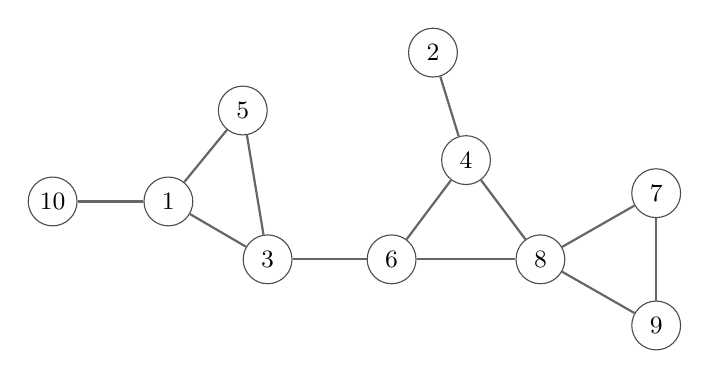
\begin{tikzpicture}[x=1.05cm, y=1.05cm]
\node[con-v] (u10) at (0,1.2) {10};
\node[con-v] (u1) at (1.4,1.2) {1};
\node[con-v] (u5) at (2.3,2.3) {5};
\node[con-v] (u3) at (2.6,0.5) {3};
\node[con-v] (u6) at (4.1,0.5) {6};
\node[con-v] (u4) at (5.0,1.7) {4};
\node[con-v] (u2) at (4.6,3.0) {2};
\node[con-v] (u8) at (5.9,0.5) {8};
\node[con-v] (u7) at (7.3,1.3) {7};
\node[con-v] (u9) at (7.3,-0.3) {9};
\draw[con-e] (u1) -- (u3);
\draw[con-e] (u1) -- (u5);
\draw[con-e] (u1) -- (u10);
\draw[con-e] (u2) -- (u4);
\draw[con-e] (u3) -- (u5);
\draw[con-e] (u3) -- (u6);
\draw[con-e] (u4) -- (u6);
\draw[con-e] (u4) -- (u8);
\draw[con-e] (u6) -- (u8);
\draw[con-e] (u7) -- (u8);
\draw[con-e] (u7) -- (u9);
\draw[con-e] (u8) -- (u9);
\end{tikzpicture}
\diagcaption{校園的大樓和走廊：$10$ 棟大樓、$12$ 條走廊。}
\label{fig:con-corridor}
\end{center}

圖~\ref{fig:con-corridor} 是章首的校園。 用眼睛看：封掉大樓 $3$，$\{1, 5, 10\}$ 和右邊
就分開了，$3$ 是割點；走廊 $3$--$6$ 是左右兩半之間唯一的一條，是橋。 大樓 $5$ 不是割
點，封掉它，$1$ 和 $3$ 之間還有走廊 $1$--$3$。 一個一個試的話，每個頂點拿掉後做一次
DFS，要 $O(n(n + m))$；每條邊試一次要 $O(m(n + m))$。 下面用一次 DFS 全部找出來。

\subsection{無向圖的 DFS 樹}

第~21~章的定理~\ref{thm:gtr-undirected} 證明過，無向圖的 DFS 只會產生\textbf{樹邊}和\textbf{後向邊}，沒有前向邊和
交叉邊。 換句話說，每一條邊的兩端，一定有一個是另一個在 DFS 樹裡的祖先。 這是本節所
有證明的基礎。 實作時有兩個細節：

\begin{itemize}
\item 無向邊在鄰接串列裡出現兩次。 從子節點 $v$ 看到父節點 $u$ 時，那是樹邊 $\{u, v\}$
本身，不是後向邊，要跳過。 簡單圖裡用「$w$ 是不是父節點」判斷就夠了。
\item 後向邊 $\{x, w\}$（$w$ 是 $x$ 的祖先）也會被看到兩次：從 $x$ 看到 $w$ 時 $w$ 是灰
色；從 $w$ 看到 $x$ 時，$x$ 已經完成。 後者 $d[x] > d[w]$，拿來更新 $\mathit{low}[w]$ 不
會改變任何值，可以不必特別排除。
\end{itemize}

令 $T(v)$ 表示 $v$ 在 DFS 樹裡的子樹。 一條邊如果一端在 $T(v)$ 裡、另一端在外面，因為
兩端有祖先關係，外面那一端一定是 $v$ 的真祖先。 所以：

\begin{lemma}
\label{lem:con-leave}
設 $v$ 是 $u$ 在 DFS 樹裡的子節點。 連接 $T(v)$ 和 $T(v)$ 以外頂點的邊只有兩種：樹邊
$\{u, v\}$，以及從 $T(v)$ 裡的頂點連到 $u$ 或 $u$ 的祖先的後向邊。
\end{lemma}

\subsection{low 值}

\begin{definition}
在無向圖的 DFS 裡，頂點 $u$ 的 $\mathit{low}[u]$ 是下面這些數的最小值：
\begin{itemize}
\item $d[u]$；
\item $\mathit{low}[v]$，$v$ 是 $u$ 的子節點；
\item $d[w]$，$\{u, w\}$ 是後向邊，$w$ 是 $u$ 的祖先（不含走下來的那條樹邊的父節點）。
\end{itemize}
\end{definition}

$d$ 的編號和第~\ref{sec:con-tarjan}~節一樣是發現順序 $1, 2, \ldots, n$。 把子節點一層
一層展開，就得到另一種寫法：
\[
\mathit{low}[u] = \min\bigl(\{d[u]\} \cup \{d[w] : x \in T(u)，\{x, w\} \text{ 是後向邊、} w \text{ 是 } x \text{ 的祖先}\}\bigr),
\]
也就是「從 $u$ 的子樹出發，往下走任意條樹邊，最後\textbf{最多走一條後向邊}，能到達的
最早發現的頂點」的 $d$ 值。 有些課本用遞迴的寫法定義，有些用「子樹裡的後向邊」定義，
兩者算出來的數字相同。 子樹裡的頂點 $d$ 都比 $u$ 大，所以 $\mathit{low}[u] < d[u]$ 表
示子樹裡有後向邊回到 $u$ 的真祖先；$\mathit{low}[u] = d[u]$ 表示沒有。

和 Tarjan 演算法比，這裡沒有堆疊：無向圖沒有交叉邊，不會碰到「已經切出去的元件」，
後向邊另一端的祖先一定還是灰色。

由引理~\ref{lem:con-leave}，對 $u$ 的子節點 $v$，後向邊離開 $T(v)$ 時只能到 $u$（$d$
值是 $d[u]$）或 $u$ 的真祖先（$d$ 值比 $d[u]$ 小），而 $T(v)$ 裡的頂點 $d$ 值都比
$d[u]$ 大。 所以：
\begin{itemize}
\item $\mathit{low}[v] \ge d[u]$ 若且唯若 $T(v)$ 沒有後向邊連到 $u$ 的\textbf{真祖先}；
\item $\mathit{low}[v] > d[u]$ 若且唯若 $T(v)$ 沒有後向邊連到 $u$ \textbf{或} $u$ 的真
祖先，也就是除了樹邊 $\{u, v\}$ 之外，沒有任何邊離開 $T(v)$。
\end{itemize}

\subsection{三個判斷規則}

\begin{theorem}[根]
\label{thm:con-root}
DFS 樹的根 $r$ 是割點，若且唯若 $r$ 在 DFS 樹裡至少有兩個子節點。
\end{theorem}

\begin{proof}
設 $r$ 有兩個子節點 $v_1$、$v_2$。 由引理~\ref{lem:con-leave}，離開 $T(v_1)$ 的邊只能
連到 $r$（$r$ 沒有祖先），所以拿掉 $r$ 後，$T(v_1)$ 和 $T(v_2)$ 之間沒有邊，分成不同的
元件，個數變多，$r$ 是割點。 反過來，$r$ 沒有子節點時 $r$ 是孤立點，拿掉後元件少一
個；$r$ 只有一個子節點 $v$ 時，$r$ 的元件拿掉 $r$ 後剩下 $T(v)$，靠樹邊就連通，元件個
數不變。 這兩種情況 $r$ 都不是割點。
\end{proof}

\begin{theorem}[非根]
\label{thm:con-nonroot}
非根的頂點 $u$ 是割點，若且唯若 $u$ 有某個子節點 $v$ 滿足 $\mathit{low}[v] \ge d[u]$。
\end{theorem}

\begin{proof}
設 $p$ 是 $u$ 的父節點，$K$ 是 $u$ 所在的連通元件（也就是這棵 DFS 樹的頂點）。

若某個子節點 $v$ 滿足 $\mathit{low}[v] \ge d[u]$：$T(v)$ 沒有後向邊連到 $u$ 的真祖先，由
引理~\ref{lem:con-leave}，離開 $T(v)$ 的邊全都接在 $u$ 上。 拿掉 $u$ 以後，$T(v)$ 和
$p$ 不再相連（$p$ 不在 $T(v)$ 裡），$K$ 至少分成兩塊，$u$ 是割點。

若每個子節點 $v$ 都滿足 $\mathit{low}[v] < d[u]$：拿掉 $u$ 後，把 $K$ 剩下的頂點分成
$R = K - T(u)$ 和各個 $T(v)$。 樹拿掉子樹 $T(u)$ 後仍然是一棵樹，所以 $R$ 靠樹邊連通，
而且 $p \in R$。 每個 $T(v)$ 自己靠樹邊連通，又有一條後向邊連到 $u$ 的真祖先，那個祖先
在 $R$ 裡。 所以 $K - u$ 仍然連通，元件個數不變，$u$ 不是割點。
\end{proof}

\begin{theorem}[橋]
\label{thm:con-bridge}
後向邊都不是橋。 樹邊 $\{u, v\}$（$u$ 是 $v$ 的父節點）是橋，若且唯若 $\mathit{low}[v]
> d[u]$。
\end{theorem}

\begin{proof}
後向邊 $\{x, w\}$ 加上樹上從 $w$ 到 $x$ 的路，構成一個環。 一條邊在環上，拿掉它以後兩
端還能沿著環的另一半相連，元件個數不變，所以不是橋。

樹邊 $\{u, v\}$：若 $\mathit{low}[v] > d[u]$，除了 $\{u, v\}$ 本身，沒有任何邊離開
$T(v)$，拿掉它，$T(v)$ 就和 $u$ 分開了，是橋。 若 $\mathit{low}[v] \le d[u]$，$T(v)$ 裡
有某個 $x$ 經後向邊連到 $w$，$w$ 是 $u$ 或 $u$ 的真祖先。 這條後向邊不是 $\{u, v\}$ 本
身（那是樹邊），所以 $w \leadsto u \to v \leadsto x \to w$ 是一個包含 $\{u, v\}$ 的環，
$\{u, v\}$ 不是橋。
\end{proof}

橋的判斷是嚴格的 $>$，非根割點的判斷是 $\ge$。 差別在「後向邊剛好回到 $u$」：這時拿掉
$u$ 會把 $T(v)$ 切開，但拿掉 $\{u, v\}$ 不會，因為 $T(v)$ 還能經過那條後向邊回到 $u$。

\begin{pseudo}[label=alg:con-cut]{割點與橋}
\Procedure{Cut-Bridge}{$G$}
    \State $\mathit{time} \gets 0$
    \State 把每個 $d[u]$ 設成 $0$、$\mathit{cut}[u]$ 設成 \FALSE
    \For{每個頂點 $u$（由小到大）}
        \If{$d[u] = 0$}
            \State \Call{Cut-Visit}{$G, u, \NIL$}
        \EndIf
    \EndFor
\EndProcedure
\Procedure{Cut-Visit}{$G, u, p$} \Comment{$p$ 是 $u$ 的父節點}
    \State $\mathit{time} \gets \mathit{time} + 1$；$d[u] \gets \mathit{time}$；$\mathit{low}[u] \gets \mathit{time}$
    \State $c \gets 0$ \Comment{子節點個數}
    \For{每個 $w \in \mathit{Adj}[u]$}
        \If{$d[w] = 0$} \Comment{樹邊}
            \State $c \gets c + 1$
            \State \Call{Cut-Visit}{$G, w, u$}
            \State $\mathit{low}[u] \gets \min(\mathit{low}[u], \mathit{low}[w])$
            \If{$p \ne \NIL$ \AND $\mathit{low}[w] \ge d[u]$}
                \State $\mathit{cut}[u] \gets \TRUE$
            \EndIf
            \If{$\mathit{low}[w] > d[u]$}
                \State 輸出橋 $\{u, w\}$
            \EndIf
        \ElsIf{$w \ne p$} \Comment{後向邊}
            \State $\mathit{low}[u] \gets \min(\mathit{low}[u], d[w])$
        \EndIf
    \EndFor
    \If{$p = \NIL$ \AND $c \ge 2$}
        \State $\mathit{cut}[u] \gets \TRUE$
    \EndIf
\EndProcedure
\end{pseudo}

第 15 行可能對同一個 $u$ 成立好幾次（$u$ 有好幾個子節點都滿足），所以用
$\mathit{cut}[u]$ 記下來，不要每次成立就把割點個數加一。 第 19--20 行的 $w$ 可能是已經完成
的子孫（後向邊從祖先那一端看到），$d[w] > d[u]$，取 $\min$ 不會改變任何值。 每條邊在
第 10 行被看兩次，總時間 $\Theta(n + m)$。

\subsection{手算追蹤}

在圖~\ref{fig:con-corridor} 上從 $1$ 開始，鄰居由小到大。 $1$ 的鄰居是 $3, 5, 10$，先走
到 $3$；$3$ 的鄰居 $1$ 是父節點，跳過，接著走到 $5$；$5$ 的鄰居 $1$ 是祖先，$\{5, 1\}$
是後向邊。 $5$ 完成，回到 $3$ 走 $6$，$6 \to 4 \to 2$；$2$ 只有父節點這個鄰居，完成；
$4$ 的下一個鄰居 $6$ 是父節點，再來 $8$；$8$ 的鄰居 $4$ 是父節點，$6$ 是祖先（後向邊
$\{8, 6\}$），接著 $8 \to 7 \to 9$，$9$ 的鄰居 $8$ 是祖先（後向邊 $\{9, 8\}$）。 一路完
成回到 $1$ 以後，$1$ 的鄰居 $5$ 已經完成（$d[5] > d[1]$，略過），最後走到 $10$。 得到
的 DFS 樹如下。

\begin{center}
\begin{tikzpicture}[x=1.0cm, y=0.95cm]
\node[con-v] (t1) at (0,0) {1};
\node[con-v] (t3) at (-1.3,-1) {3};
\node[con-v] (t10) at (1.3,-1) {10};
\node[con-v] (t5) at (-2.4,-2) {5};
\node[con-v] (t6) at (-0.4,-2) {6};
\node[con-v] (t4) at (-0.4,-3) {4};
\node[con-v] (t2) at (-1.4,-4) {2};
\node[con-v] (t8) at (0.6,-4) {8};
\node[con-v] (t7) at (0.6,-5) {7};
\node[con-v] (t9) at (0.6,-6) {9};
\draw[con-tree] (t1) -- (t3);
\draw[con-tree] (t1) -- (t10);
\draw[con-tree] (t3) -- (t5);
\draw[con-tree] (t3) -- (t6);
\draw[con-tree] (t6) -- (t4);
\draw[con-tree] (t4) -- (t2);
\draw[con-tree] (t4) -- (t8);
\draw[con-tree] (t8) -- (t7);
\draw[con-tree] (t7) -- (t9);
\draw[con-back] (t5) to[bend left=65] (t1);
\draw[con-back] (t8) to[bend right=45] (t6);
\draw[con-back] (t9) to[bend right=50] (t8);
\node[con-lab, right=1mm of t1] {1/1};
\node[con-lab, above left=0.3mm of t3] {2/1};
\node[con-lab, right=1mm of t10] {10/10};
\node[con-lab, left=1mm of t5] {3/1};
\node[con-lab, left=1mm of t6] {4/4};
\node[con-lab, left=1mm of t4] {5/4};
\node[con-lab, left=1mm of t2] {6/6};
\node[con-lab, left=1mm of t8] {7/4};
\node[con-lab, left=1mm of t7] {8/7};
\node[con-lab, left=1mm of t9] {9/7};
\end{tikzpicture}
\diagcaption{圖~\ref{fig:con-corridor} 從 $1$ 開始的 DFS 樹。 粗線是樹邊，虛線是後向
邊；每個頂點旁邊是 $d/\mathit{low}$。}
\label{fig:con-corridor-tree}
\end{center}

$\mathit{low}$ 要從葉節點往上算：子節點的 $\mathit{low}$ 算好，父節點才能算。 下表依 $d$
排列，最後一欄是每條樹邊 $\{u, v\}$ 的判斷（$v$ 是子節點）。

\begin{center}
\small
\setlength{\tabcolsep}{4pt}
\begin{tabular}{ccccc>{\raggedright\arraybackslash}p{0.44\linewidth}}
\toprule
$u$ & $d$ & 子節點 & 後向邊到 & $\mathit{low}$ & 判斷 \\
\midrule
1 & 1 & 3, 10 & — & $\min(1, 1, 10) = 1$ & 根，兩個子節點：割點 \\
3 & 2 & 5, 6 & — & $\min(2, 1, 4) = 1$ & $\mathit{low}[6] = 4 \ge 2$：割點；$4 > 2$：$\{3, 6\}$ 是橋 \\
5 & 3 & — & 1 & $\min(3, d[1]) = 1$ & 葉節點 \\
6 & 4 & 4 & — & $\min(4, 4) = 4$ & $\mathit{low}[4] = 4 \ge 4$：割點；$4 \not> 4$：不是橋 \\
4 & 5 & 2, 8 & — & $\min(5, 6, 4) = 4$ & $\mathit{low}[2] = 6 \ge 5$：割點；$6 > 5$：$\{4, 2\}$ 是橋 \\
2 & 6 & — & — & $6$ & 葉節點 \\
8 & 7 & 7 & 6 & $\min(7, d[6], 7) = 4$ & $\mathit{low}[7] = 7 \ge 7$：割點；不是橋 \\
7 & 8 & 9 & — & $\min(8, 7) = 7$ & $\mathit{low}[9] = 7 < 8$ \\
9 & 9 & — & 8 & $\min(9, d[8]) = 7$ & 葉節點 \\
10 & 10 & — & — & $10$ & 葉節點；$\mathit{low}[10] = 10 > 1$：$\{1, 10\}$ 是橋 \\
\bottomrule
\end{tabular}
\end{center}

結果：割點是 $1, 3, 4, 6, 8$，橋是 $\{1, 10\}$、$\{3, 6\}$、$\{2, 4\}$。 幾個要注意的地方：

\begin{itemize}
\item $3$ 有兩個子節點，$5$ 那邊有後向邊回到 $1$（$\mathit{low}[5] = 1 < 2$），$6$ 那邊沒
有。 只要\textbf{有一個}子節點滿足條件就是割點。
\item $6$ 和 $8$ 都是「$\mathit{low}[v] = d[u]$」的情況：子樹的後向邊剛好回到 $u$，$u$
是割點，但邊 $\{u, v\}$ 不是橋。
\item $4$ 和 $6$ 都是割點，但 $\{4, 6\}$ 不是橋。 兩端都是割點的邊不一定是橋；反過來，
橋的兩端也不一定都是割點，例如 $\{1, 10\}$ 的 $10$ 是葉節點。 DFS 樹的葉節點沒有子節點，定理~\ref{thm:con-nonroot} 的條件不會成立，所以一定不是割點。
\item 根 $1$ 不能用非根的規則：對子節點 $3$，$\mathit{low}[3] = 1 \ge d[1]$ 永遠成立，根
要另外數子節點。
\end{itemize}

\begin{center}
\begin{tikzpicture}[x=1.05cm, y=1.05cm]
\node[con-v] (u10) at (0,1.2) {10};
\node[con-v, con-cut] (u1) at (1.4,1.2) {1};
\node[con-v] (u5) at (2.3,2.3) {5};
\node[con-v, con-cut] (u3) at (2.6,0.5) {3};
\node[con-v, con-cut] (u6) at (4.1,0.5) {6};
\node[con-v, con-cut] (u4) at (5.0,1.7) {4};
\node[con-v] (u2) at (4.6,3.0) {2};
\node[con-v, con-cut] (u8) at (5.9,0.5) {8};
\node[con-v] (u7) at (7.3,1.3) {7};
\node[con-v] (u9) at (7.3,-0.3) {9};
\draw[con-e] (u1) -- (u3);
\draw[con-e] (u1) -- (u5);
\draw[con-bridge] (u1) -- (u10);
\draw[con-bridge] (u2) -- (u4);
\draw[con-e] (u3) -- (u5);
\draw[con-bridge] (u3) -- (u6);
\draw[con-e] (u4) -- (u6);
\draw[con-e] (u4) -- (u8);
\draw[con-e] (u6) -- (u8);
\draw[con-e] (u7) -- (u8);
\draw[con-e] (u7) -- (u9);
\draw[con-e] (u8) -- (u9);
\end{tikzpicture}
\diagcaption{校園的割點（橘色）和橋（紅色粗線）。}
\label{fig:con-corridor-cut}
\end{center}

\begin{examnote}
$\mathit{low}$ 的手算表各課本寫法不同，作答前先看題目的約定。 (1) $d$ 的編號有的從
$0$ 開始，有的用第~21~章同時記 $d$、$f$ 的時間戳記，數字會不同，但判斷只比大小，割
點、橋的結果一樣。 (2) 遞迴的定義和「子樹裡的後向邊」的定義算出來的數字相同。 (3) 有
的程式在後向邊寫 $\mathit{low}[u] \gets \min(\mathit{low}[u], \mathit{low}[w])$，用
$\mathit{low}[w]$ 代替 $d[w]$。 祖先 $w$ 這時的 $\mathit{low}$ 可能已經比 $d[w]$ 小，算
出的數字就會變小：上例 $8$ 先處理後向邊 $\{8, 6\}$，$\mathit{low}[8]$ 已經是 $4$，之後
$9$ 的後向邊 $\{9, 8\}$ 會讓 $\mathit{low}[9] = \mathit{low}[7] = 4$，$\mathit{low}[7] = 4
< d[8] = 7$，\textbf{割點 $8$ 就找不到了}。 這種寫法找橋的結果仍然正確，找割點會錯，
作答時一律用 $d[w]$。（Tarjan 強連通元件演算法做同樣的替換，數字也會變，但找到的元件不
變，見觀念題第~\ref{q:con-variant-proof}~題。）
\end{examnote}

\subsection{平行邊}

如果兩棟大樓之間有兩條走廊，拿掉其中一條還有另一條，它們都不是橋。 但虛擬碼第 19 行
用「$w \ne p$」判斷，會把兩條都當成走下來的樹邊跳過，$\mathit{low}[v]$ 算大了，就把
$\{u, v\}$ 誤判成橋。 有平行邊時，要幫每條邊編號，遞迴時傳「走下來的那條邊的編號」，
只跳過那一條，其他連回父節點的邊照樣當後向邊。 割點不受影響：回到父節點 $u$ 的後向邊
最多讓 $\mathit{low}[v]$ 降到 $d[u]$，$\mathit{low}[v] \ge d[u]$ 的判斷結果不變。

\section{雙連通元件}
\label{sec:con-bcc}

割點把圖分成幾塊，每一塊內部「封掉任何一棟大樓都還走得通」。 這些塊就是雙連通元件。

\begin{definition}
無向圖裡兩條邊 $e_1$、$e_2$，如果 $e_1 = e_2$，或者有一個\textbf{簡單環}（頂點不重複
的環）同時經過 $e_1$ 和 $e_2$，就說它們屬於同一塊。 這是一個等價關係，它把所有的邊分
成若干類，每一類叫做一個\textbf{雙連通元件}（biconnected component），也叫\textbf{區
塊}（block）。
\end{definition}

自反（$e_1 = e_1$）和對稱（同一個環也同時經過 $e_2$、$e_1$）直接從定義看得出來；遞移性（$e_1, e_2$ 在同一個環上、$e_2, e_3$ 在同一個環上，則
$e_1, e_3$ 也在某個環上）需要一點功夫，這裡不證，見延伸閱讀。 幾個常用的性質：

\begin{itemize}
\item 橋不在任何環上，所以每一座橋自己是一個區塊。
\item 兩個不同的區塊最多共用一個頂點，共用的頂點一定是割點（觀念題第~\ref{q:con-block-share}~題）。
\item 一個頂點是割點，若且唯若它屬於兩個以上的區塊。
\end{itemize}

有的課本改用頂點定義：沒有割點的連通圖叫\textbf{雙連通圖}（只有一條邊、兩個頂點的
圖也算），雙連通元件是最大的雙連通子圖。 兩種定義對有邊的部分得到同樣的分法；差別只在孤立
頂點，頂點定義把它算成一個元件，邊定義不算。

圖~\ref{fig:con-corridor-cut} 的校園有 $6$ 個區塊：
\[
\{2\text{--}4\},\ \{7\text{--}8, 7\text{--}9, 8\text{--}9\},\ \{4\text{--}6, 4\text{--}8, 6\text{--}8\},\
\{3\text{--}6\},\ \{1\text{--}3, 1\text{--}5, 3\text{--}5\},\ \{1\text{--}10\}.
\]
每個割點都
剛好落在兩個區塊的交界：$4$ 在第一、三塊，$8$ 在第二、三塊，$6$ 在第三、四塊，$3$ 在第
四、五塊，$1$ 在第五、六塊。

\subsection{用邊的堆疊找區塊}

在割點演算法上加一個\textbf{邊的堆疊}就能把區塊切出來，想法和 Tarjan 強連通元件演算
法一樣：DFS 走過的邊依序推進堆疊；當子節點 $w$ 做完、發現 $\mathit{low}[w] \ge d[u]$
時，$u$ 把 $T(w)$ 這一側和圖的其他部分隔開，堆疊上從樹邊 $(u, w)$ 以上、還沒被彈出的
邊，就是一個區塊。

\begin{pseudo}[label=alg:con-bcc]{雙連通元件（主程序和虛擬碼~\ref{alg:con-cut} 相同，另外設 $S \gets$ 空堆疊、$k \gets 0$）}
\Procedure{BCC-Visit}{$G, u, p$}
    \State $\mathit{time} \gets \mathit{time} + 1$；$d[u] \gets \mathit{time}$；$\mathit{low}[u] \gets \mathit{time}$
    \For{每個 $w \in \mathit{Adj}[u]$}
        \If{$d[w] = 0$} \Comment{樹邊}
            \State \Call{Push}{$S, (u, w)$}
            \State \Call{BCC-Visit}{$G, w, u$}
            \State $\mathit{low}[u] \gets \min(\mathit{low}[u], \mathit{low}[w])$
            \If{$\mathit{low}[w] \ge d[u]$}
                \State $k \gets k + 1$ \Comment{新的區塊}
                \Repeat
                    \State $(x, y) \gets$ \Call{Pop}{$S$}；把邊 $\{x, y\}$ 標成第 $k$ 個區塊
                \Until{$(x, y) = (u, w)$}
            \EndIf
        \ElsIf{$w \ne p$ \AND $d[w] < d[u]$} \Comment{往祖先的後向邊}
            \State \Call{Push}{$S, (u, w)$}
            \State $\mathit{low}[u] \gets \min(\mathit{low}[u], d[w])$
        \EndIf
    \EndFor
\EndProcedure
\end{pseudo}

和虛擬碼~\ref{alg:con-cut} 比，有三個差別。 第一，第 13 行多了 $d[w] < d[u]$：後向邊從
祖先那一端看到時不能再推一次，否則同一條邊會進堆疊兩次。 第二，第 8 行的判斷\textbf{包
含根}：根的每個子節點都會切出區塊，根有兩個子節點時就切出兩組，這正好對應「根是割點」。
第三，每條邊恰好進出堆疊各一次，所以總時間仍然是 $\Theta(n + m)$，堆疊最多放 $m$ 條邊。

為什麼一次彈出的剛好是一個區塊？ 完整的證明比較長，這裡只說想法。 對彈出的先後做歸
納：$T(w)$ 裡比較深的地方，凡是被某個割點隔開的部分，都在更早的時候被彈走了；留下
來的邊，每一條都能透過子樹裡的後向邊和 $(u, w)$ 繞成環，所以都在同一個區塊。 另一方
面，$\mathit{low}[w] \ge d[u]$ 表示 $T(w)$ 沒有邊越過 $u$ 往上，$u$ 以上的邊和這些邊不可
能在同一個環上，所以這一塊不會再變大。

\subsection{手算追蹤}

DFS 的走法和圖~\ref{fig:con-corridor-tree} 相同。 邊寫成 $u$--$w$ 表示從 $u$ 看到 $w$
時推進堆疊（樹邊由父到子，後向邊由子孫到祖先）。 只有判斷成立的六個時刻會彈出：

\begin{center}
\small
\setlength{\tabcolsep}{4pt}
\begin{tabular}{ll>{\raggedright\arraybackslash}p{0.42\linewidth}l}
\toprule
時刻 & 判斷 & 彈出前的堆疊（底 $\to$ 頂） & 彈出的區塊 \\
\midrule
從 $2$ 回到 $4$ & $\mathit{low}[2] = 6 \ge 5$ & \mbox{1--3}, \mbox{3--5}, \mbox{5--1}, \mbox{3--6}, \mbox{6--4}, \mbox{4--2} & \mbox{4--2} \\
從 $7$ 回到 $8$ & $\mathit{low}[7] = 7 \ge 7$ & \mbox{1--3}, \mbox{3--5}, \mbox{5--1}, \mbox{3--6}, \mbox{6--4}, \mbox{4--8}, \mbox{8--6}, \mbox{8--7}, \mbox{7--9}, \mbox{9--8} & \mbox{9--8}, \mbox{7--9}, \mbox{8--7} \\
從 $4$ 回到 $6$ & $\mathit{low}[4] = 4 \ge 4$ & \mbox{1--3}, \mbox{3--5}, \mbox{5--1}, \mbox{3--6}, \mbox{6--4}, \mbox{4--8}, \mbox{8--6} & \mbox{8--6}, \mbox{4--8}, \mbox{6--4} \\
從 $6$ 回到 $3$ & $\mathit{low}[6] = 4 \ge 2$ & \mbox{1--3}, \mbox{3--5}, \mbox{5--1}, \mbox{3--6} & \mbox{3--6} \\
從 $3$ 回到 $1$ & $\mathit{low}[3] = 1 \ge 1$ & \mbox{1--3}, \mbox{3--5}, \mbox{5--1} & \mbox{5--1}, \mbox{3--5}, \mbox{1--3} \\
從 $10$ 回到 $1$ & $\mathit{low}[10] = 10 \ge 1$ & \mbox{1--10} & \mbox{1--10} \\
\bottomrule
\end{tabular}
\end{center}

其他幾次回到父節點時判斷都不成立：從 $5$ 回到 $3$（$\mathit{low}[5] = 1 < 2$）、從 $8$
回到 $4$（$4 < 5$）、從 $9$ 回到 $7$（$7 < 8$）。 這些邊留在堆疊上，等上面的頂點一起
彈出。 注意第二列：$4$--$8$ 比 $8$--$6$ 早進堆疊，但它不屬於第二個區塊，彈到 $8$--$7$
就停了，$4$--$8$ 和 $8$--$6$ 留給第三列。

\begin{examnote}
雙連通元件的答案可以寫成邊的集合，也可以寫成頂點的集合（例如第三塊是 $\{4, 6, 8\}$）；
寫頂點時，割點會同時出現在好幾塊裡，這是正常的。 題目用頂點定義、圖裡又有孤立頂點時，
每個孤立頂點自己算一塊，邊的堆疊不會產生它，要另外補上。 有的題目只問區塊個數，就是
第 8 行成立的次數。
\end{examnote}

\subsection{C 程式}

下面的程式把本章無向圖的三件事一次做完：照虛擬碼~\ref{alg:con-bcc} 的走法，在判斷成
立時印出區塊（如果同時 $\mathit{low}[w] > d[u]$，先印出橋），最後印出每個頂點的 $d$、
$\mathit{low}$ 和所有割點。 每條無向邊在鄰接串列裡加兩次。 邊的堆疊是一個
\texttt{Edge} 陣列，最多放 $m$ 條邊；\texttt{(Edge)\{u, w\}} 是 C99 起的複合字面值，直接
造出一個結構值。 輸入是圖~\ref{fig:con-corridor} 的校園。

\begin{example}[label=ex:con-cut]{c}{(cut\_bridge.c) 割點、橋與雙連通元件}
#include <stdio.h>
#include <stdlib.h>

typedef struct Node {
    int v;
    struct Node *next;
} Node;

typedef struct {
    int n;
    Node **adj;     // adj[u]：u 的鄰居，由小到大
} Graph;

int add_arc(Graph *g, int u, int v)
{
    Node *x = malloc(sizeof *x);
    if (x == NULL) {
        return 0;
    }
    Node **p = &g->adj[u];
    while (*p != NULL && (*p)->v < v) {
        p = &(*p)->next;
    }
    x->v = v;
    x->next = *p;
    *p = x;
    return 1;
}

void free_graph(Graph *g)
{
    for (int u = 0; g->adj != NULL && u < g->n; u++) {
        Node *x = g->adj[u];
        while (x != NULL) {
            Node *next = x->next;
            free(x);
            x = next;
        }
    }
    free(g->adj);
}

typedef struct {
    int u, w;
} Edge;

typedef struct {
    const Graph *g;
    int *d, *low;       // d[u] = 0 表示還沒發現
    int *is_cut;
    Edge *es;           // 邊的堆疊
    int top, time, blocks;
} Search;

void visit(Search *s, int u, int parent)
{
    s->d[u] = s->low[u] = ++s->time;
    int children = 0;
    for (Node *x = s->g->adj[u]; x != NULL; x = x->next) {
        int w = x->v;
        if (s->d[w] == 0) {                         // 樹邊
            children++;
            s->es[s->top++] = (Edge){u, w};
            visit(s, w, u);
            if (s->low[w] < s->low[u]) {
                s->low[u] = s->low[w];
            }
            if (s->low[w] >= s->d[u]) {     // w 的子樹到不了 u 上面
                if (parent != -1) {
                    s->is_cut[u] = 1;
                }
                if (s->low[w] > s->d[u]) {
                    printf("bridge %d-%d\n", u + 1, w + 1);
                }
                printf("block %d:", ++s->blocks);
                Edge e;
                do {
                    e = s->es[--s->top];
                    printf(" %d-%d", e.u + 1, e.w + 1);
                } while (e.u != u || e.w != w);
                printf("\n");
            }
        } else if (w != parent && s->d[w] < s->d[u]) {  // 後向邊
            s->es[s->top++] = (Edge){u, w};
            if (s->d[w] < s->low[u]) {
                s->low[u] = s->d[w];
            }
        }
    }
    if (parent == -1 && children >= 2) {
        s->is_cut[u] = 1;
    }
}

int main(void)
{
    int n, m;
    if (scanf("%d %d", &n, &m) != 2 || n <= 0 || m < 0) {
        return 1;
    }
    Graph g = {n, calloc(n, sizeof(Node *))};
    Search s = {&g, calloc(n, sizeof(int)), calloc(n, sizeof(int)),
                calloc(n, sizeof(int)),
                malloc((m + 1) * sizeof(Edge)), 0, 0, 0};
    int ok = g.adj != NULL && s.d != NULL && s.low != NULL
             && s.is_cut != NULL && s.es != NULL;
    for (int i = 0; ok && i < m; i++) {
        int u, v;
        ok = scanf("%d %d", &u, &v) == 2 && u >= 1 && u <= n
             && v >= 1 && v <= n && u != v
             && add_arc(&g, u - 1, v - 1)
             && add_arc(&g, v - 1, u - 1);
    }
    if (ok) {
        for (int u = 0; u < n; u++) {
            if (s.d[u] == 0) {
                visit(&s, u, -1);
            }
        }
        printf("v:");
        for (int u = 0; u < n; u++) {
            printf(" %d", u + 1);
        }
        printf("\nd:");
        for (int u = 0; u < n; u++) {
            printf(" %d", s.d[u]);
        }
        printf("\nlow:");
        for (int u = 0; u < n; u++) {
            printf(" %d", s.low[u]);
        }
        printf("\ncut vertices:");
        for (int u = 0; u < n; u++) {
            if (s.is_cut[u]) {
                printf(" %d", u + 1);
            }
        }
        printf("\n");
    }
    free_graph(&g);
    free(s.d);
    free(s.low);
    free(s.is_cut);
    free(s.es);
    return ok ? 0 : 1;
}
\end{example}
\iosample{10 12 \\ 1 3 \\ 1 5 \\ 1 10 \\ 2 4 \\ 3 5 \\ 3 6 \\ 4 6 \\ 4 8 \\ 6 8 \\ 7 8 \\ 7 9 \\ 8 9}{bridge 4-2 \\ block 1: 4-2 \\ block 2: 9-8 7-9 8-7 \\ block 3: 8-6 4-8 6-4 \\ bridge 3-6 \\ block 4: 3-6 \\ block 5: 5-1 3-5 1-3 \\ bridge 1-10 \\ block 6: 1-10 \\ v: 1 2 3 4 5 6 7 8 9 10 \\ d: 1 6 2 5 3 4 8 7 9 10 \\ low: 1 6 1 4 1 4 7 4 7 10 \\ cut vertices: 1 3 4 6 8}

輸出和手算一致。 程式只在 $d[w] < d[u]$ 時處理後向邊，所以「從祖先那一端看到已完成的子
孫」的情況直接略過，連 $\mathit{low}$ 都不用更新。 \texttt{is\_cut} 是旗標陣列，同一個
頂點被好幾個子節點判斷成割點也只記一次。 程式假設輸入是簡單圖（讀入時擋掉了自環，平
行邊沒有檢查）。

把所有的橋拿掉，剩下的每個連通元件叫做\textbf{邊雙連通元件}（2-edge-connected
component）：裡面拿掉任何一條邊都還連通。 校園的例子拿掉三座橋後剩下 $\{1, 3, 5\}$、
$\{4, 6, 7, 8, 9\}$、$\{2\}$、$\{10\}$ 四塊。 注意 $\{4, 6, 7, 8, 9\}$ 包含兩個區塊：
邊雙連通只管邊，不管割點。

\section{本章常見錯誤}
\label{sec:con-pitfalls}

\begin{center}
\small
\begin{tabular}{>{\raggedright\arraybackslash}p{0.24\linewidth}>{\raggedright\arraybackslash}p{0.52\linewidth}>{\raggedright\arraybackslash}p{0.14\linewidth}}
\toprule
錯誤 & 例子 & 見 \\
\midrule
第二次 DFS 在 $G$ 上做 & Kosaraju 的第二次 DFS 沒有轉置，從 $7$ 出發就走遍全圖，四個元件併成一個 &
第~\ref{sec:con-kosaraju}~節 \\
挑起點的順序錯 & 第二次 DFS 照 $f$ 由小到大，或照 $d$、照編號挑起點 & 第~\ref{sec:con-kosaraju}~節 \\
沒檢查 $\mathit{onstack}$ & Tarjan 處理 $3 \to 5$ 時，$5$ 已經彈出還拿 $d[5]$ 更新，$\{3, 8\}$ 沒有被切出來 &
第~\ref{sec:con-tarjan}~節 \\
用灰色代替「在堆疊上」 & $4 \to 2$ 的 $2$ 已是黑色但還在堆疊上，只看灰色會讓 $\mathit{low}[4]$ 留在
$6$，$4$ 被誤判成頭 & 第~\ref{sec:con-tarjan}~節 \\
拿 $\mathit{low}$ 當元件編號 & $\mathit{low}[4] = 2$，但 $4$ 的元件的頭是 $1$ & 第~\ref{sec:con-tarjan}~節 \\
父節點的邊當成後向邊 & 無向圖沒有跳過父節點：每個 $\mathit{low}[v] \le d[u]$，一座橋都找不到（割點
不受影響） & 第~\ref{sec:con-cut}~節 \\
根用非根的規則 & 對根來說 $\mathit{low}[v] \ge d[r]$ 永遠成立，每個有子節點的根都被當成割點 &
定理~\ref{thm:con-root} \\
橋寫成 $\ge$ & 校園的 $\{6, 4\}$、$\{8, 7\}$ 被誤判成橋 & 定理~\ref{thm:con-bridge} \\
割點重複計數 & $u$ 有兩個子節點都滿足 $\mathit{low}[v] \ge d[u]$，割點個數加兩次 &
第~\ref{sec:con-cut}~節 \\
後向邊用 $\mathit{low}[w]$ & 校園的割點 $8$ 找不到 & 第~\ref{sec:con-cut}~節作答提醒 \\
有平行邊還用 $w \ne p$ & 兩條走廊連同一對大樓，被誤判成橋 & 第~\ref{sec:con-cut}~節 \\
後向邊推兩次 & 雙連通元件的邊堆疊沒有限制 $d[w] < d[u]$，同一條邊出現在兩個區塊 &
第~\ref{sec:con-bcc}~節 \\
遞迴太深 & 頂點排成很長的鏈時，遞迴的 DFS 用光呼叫堆疊 & 第~\ref{sec:gtr-dfs-iter}~節 \\
\bottomrule
\end{tabular}
\end{center}

\section{觀念題}
\label{sec:con-exercises}

題型和研究所考試、期中期末考的筆試相近。 沒有特別說明時，鄰接串列的鄰居依字母（或編號）
由小到大，主迴圈也從最小的頂點開始；Tarjan 演算法和割點演算法的 $d$ 是發現順序
$1, 2, \ldots$；無向圖是簡單圖。 解答在本章最後。

第~\ref{q:con-kosaraju}--\ref{q:con-dag-h} 題用同一張有向圖 $H$，頂點 $a$ 到 $h$，$14$ 條邊：
\[
\begin{array}{lllllll}
a \to d & a \to e & a \to h & b \to d & b \to e & c \to e & c \to f \\
d \to e & e \to a & e \to b & e \to g & f \to c & h \to d & h \to g
\end{array}
\]

\begin{enumerate}
\item \label{q:con-choice}（選擇，可能不只一個答案）下列哪些敘述正確？
\begin{enumerate}
\item Kosaraju 演算法的第二次 DFS 改在原圖 $G$ 上做，仍然依 $f$ 由大到小挑起點，結果一樣
正確。
\item Tarjan 演算法裡，頂點 $u$ 完成時若 $\mathit{low}[u] = d[u]$，則 $u$ 是它的強連通元件
裡最先被發現的頂點。
\item 元件圖可能有環，但不會有自環。
\item 連通的無向圖裡，兩端都是割點的邊一定是橋。
\item 至少有 $3$ 個頂點的連通無向圖如果有橋，就一定有割點。
\item 無向圖的 DFS 樹裡，沒有子節點的頂點一定不是割點。
\item 非根頂點 $u$ 有子節點 $v$ 滿足 $\mathit{low}[v] = d[u]$，則 $\{u, v\}$ 是橋。
\end{enumerate}

\item \label{q:con-kosaraju}（追蹤）對 $H$ 執行 Kosaraju 演算法。 (a) 寫出第一次 DFS 每個
頂點的 $d/f$（第~21~章的時間戳記），並把每條邊分類。 (b) 寫出依 $f$ 由大到小的順序和
$H^{\mathrm{T}}$ 的鄰接串列。 (c) 寫出第二次 DFS 的每一棵樹。

\item \label{q:con-tarjan-h}（追蹤）對 $H$ 執行 Tarjan 演算法（虛擬碼~\ref{alg:con-tarjan}）。
(a) 寫出每個頂點的 $d$、$\mathit{low}$，以及元件被彈出的順序。 (b) 如果第 15 行改成
$\mathit{low}[u] \gets \min(\mathit{low}[u], \mathit{low}[w])$，哪些頂點的 $\mathit{low}$
會改變？ 輸出的元件有沒有改變？（第~\ref{q:con-variant-proof} 題證明一般的情形。）

\item \label{q:con-dag-h}（計算）(a) 畫出 $H$ 的元件圖，寫出一個拓樸順序。 (b) 從哪些頂點出
發可以到達所有頂點？ (c) 把邊 $c \to e$ 刪掉，至少要選幾個起點才能到達所有頂點？ 舉一組。

\item \label{q:con-variant-proof}（證明）證明：把 Tarjan 演算法第 15 行的 $d[w]$ 換成
$\mathit{low}[w]$，找到的強連通元件和彈出的順序都不變。（提示：令新的值是
$\mathit{low}'$。 證明 $\mathit{low}'[u] \le \mathit{low}[u]$，以及 $\mathit{low}'[u] \ge
d[h(u)]$，其中 $h(u)$ 是 $u$ 的元件的頭。）

\item （計算）(a) $n$ 個頂點的有向圖有 $k$ 個強連通元件，元件圖最多有幾條邊？ (b) $n \ge 2$
個頂點的強連通有向圖最少有幾條邊？ 證明你的答案。 (c) 對一個 DAG 執行 Tarjan 演算法，
每個元件有幾個頂點？ 元件被彈出的順序和第~22~章的拓樸排序有什麼關係？

\item \label{q:con-cut-k}（追蹤）無向圖 $K$ 有頂點 $a$ 到 $i$ 和下面 $12$ 條邊：
\[
\begin{array}{llllll}
a\text{--}e & a\text{--}g & a\text{--}i & b\text{--}f & b\text{--}h & c\text{--}f \\
d\text{--}h & d\text{--}i & e\text{--}g & f\text{--}h & g\text{--}i & h\text{--}i
\end{array}
\]
從 $a$ 開始做 DFS。 (a) 畫出 DFS 樹和後向邊，寫出每個頂點的 $d$ 和 $\mathit{low}$。 (b) 找
出所有割點和橋。 (c) 用虛擬碼~\ref{alg:con-bcc} 依序寫出彈出的區塊。

\item （追蹤）承上題，如果後向邊改用 $\mathit{low}[u] \gets \min(\mathit{low}[u],
\mathit{low}[w])$，哪些頂點的 $\mathit{low}$ 會改變？ 用非根規則會找到哪些割點？ 橋呢？

\item \label{q:con-block-share}（證明）證明：簡單無向圖裡，兩個不同的區塊最多共用一個頂點，而且共用的頂點一定是割點。

\item （追蹤）四棟大樓 $1, 2, 3, 4$ 之間有五條走廊：$1$--$2$ 有兩條，另外是 $2$--$3$、
$3$--$4$、$2$--$4$。 (a) 正確的割點和橋是哪些？ (b) 直接用虛擬碼~\ref{alg:con-cut}
（第 19 行判斷 $w \ne p$），從 $1$ 開始會輸出什麼？ (c) 怎麼改才對？

\item （證明）(a) 一個連通的簡單無向圖有割點、但沒有橋，最少有幾個頂點？ 畫出一個例子，
並證明不能更少。 (b) 舉一個有橋、但沒有割點的連通圖。
\end{enumerate}

\section{實作練習}
\label{sec:con-practice}

下面是 Aki-Judge 上和本章相關的題目。 強連通元件本身目前沒有題目，可以用範
例~\ref{ex:con-tarjan} 自己出幾張圖練習，再和手算對照。

\begin{center}
\begin{tabular}{llc}
\toprule
小節 & 題目 & 難度 \\
\midrule
割點 & \akiref{count-cut-vertices}{割點個數} & 基本 \\
橋 & \akiref{count-bridge-edges}{橋邊個數} & 基本 \\
雙連通元件 & \akiref{count-biconnected-blocks}{雙連通區塊個數} & 進階 \\
縮點 & \akiref{count-reachable-pairs}{可達點對個數} & 進階 \\
\bottomrule
\end{tabular}
\end{center}

幾題的提示：

\begin{itemize}
\item 「割點個數」的圖不一定連通，主迴圈要從每個還沒發現的頂點各做一次 DFS，每棵樹的根
都用根的規則。 同一個頂點可能被好幾個子節點判斷成割點，用旗標陣列記，最後再數。
\item 「橋邊個數」照定理~\ref{thm:con-bridge}，用 $\mathit{low}[v] > d[u]$。 題目保證沒有平
行邊，跳過父節點就好。
\item 「雙連通區塊個數」只問個數，不用真的存邊的堆疊：數虛擬碼~\ref{alg:con-bcc} 第 8 行成
立幾次（包含根）。 沒有邊的孤立頂點不算。
\item 「可達點對個數」的 $n$ 很小，從每個頂點各做一次 DFS 數走得到的頂點就夠快，總共
$O(n(n + m))$。 用本章的想法可以再省：同一個強連通元件裡的頂點能到達的集合一樣，每個元
件只要算一次，再乘上元件的大小。 第~25~章的遞移閉包是另一種做法。
\end{itemize}

\section{讀完你應該會}
\label{sec:con-checklist}

\begin{itemize}
\item 說出強連通元件、元件圖的定義，證明元件圖沒有環，知道 $G$ 和 $G^{\mathrm{T}}$ 的元件
相同。
\item 手算 Kosaraju 演算法：第一次 DFS 的 $d/f$、依 $f$ 由大到小的順序、第二次在
$G^{\mathrm{T}}$ 上的每一棵樹，並用完成時間的引理說明它為什麼對。
\item 手算 Tarjan 演算法的 $d$、$\mathit{low}$ 和堆疊，說明為什麼要檢查「在不在堆疊上」，
以及為什麼 $\mathit{low}[u] = d[u]$ 就是元件的頭。
\item 把元件縮成 DAG，知道 Kosaraju 依拓樸順序、Tarjan 依反向拓樸順序產生元件，用源點
個數回答「從哪裡出發能到每個頂點」。
\item 在無向圖上填 $d$、$\mathit{low}$ 表，用根的規則、$\mathit{low}[v] \ge d[u]$、
$\mathit{low}[v] > d[u]$ 找割點和橋，並證明這三個規則。
\item 用邊的堆疊切出雙連通元件，知道不同課本 $\mathit{low}$ 的寫法哪些等價、哪些會算錯割點。
\end{itemize}

\textbf{延伸閱讀}（書末會整理完整的參考資料）

\begin{itemize}
\item Thomas H. Cormen 等，\textit{Introduction to Algorithms}，第 4 版，20.5 節：用兩次
DFS 求強連通元件，附元件圖和完成時間的引理；第 20 章章末的問題 20-2 用一連串小題帶出割點、
橋和雙連通元件。
\item Robert E. Tarjan，``Depth-First Search and Linear Graph Algorithms''，\textit{SIAM
Journal on Computing} 1(2)，1972：一次 DFS 求強連通元件和雙連通元件的原始論文。
\item M. Sharir，``A Strong-Connectivity Algorithm and Its Applications in Data Flow
Analysis''，\textit{Computers and Mathematics with Applications} 7(1)，1981：兩次 DFS 的做
法；Aho、Hopcroft、Ullman 的 \textit{Data Structures and Algorithms}（1983）把它歸功於
Kosaraju 未發表的筆記，所以常叫 Kosaraju 演算法。
\item John E. Hopcroft、Robert E. Tarjan，``Algorithm 447: Efficient Algorithms for Graph
Manipulation''，\textit{Communications of the ACM} 16(6)，1973：雙連通元件的線性時間
演算法。
\item K. P. Eswaran、R. E. Tarjan，``Augmentation Problems''，\textit{SIAM Journal on
Computing} 5(4)，1976：最少加幾條邊讓圖變成強連通或雙連通。
\item Bengt Aspvall、Michael F. Plass、Robert E. Tarjan，``A Linear-Time Algorithm for
Testing the Truth of Certain Quantified Boolean Formulas''，\textit{Information
Processing Letters} 8(3)，1979：用強連通元件解 2-SAT。
\item Steven S. Skiena，\textit{The Algorithm Design Manual}，第 3 版，7.9、7.10 節：割點和強
連通元件的另一種講法，偏重怎麼想到要用 DFS。
\end{itemize}

\addcontentsline{toc}{section}{觀念題解答}
\section*{觀念題解答}

\begin{enumerate}
\item (b)、(e)、(f) 正確。
(a)：圖~\ref{fig:con-roads} 裡 $f$ 最大的是 $7$，在 $G$ 上從 $7$ 出發會走遍全部 $9$ 個頂
點，四個元件併成一棵樹。 在 $G$ 上改照 $f$ 由小到大挑起點也不對：三個頂點、邊 $1 \to 2$、
$2 \to 1$、$1 \to 3$，第一次 DFS 得到 $f[2] = 3$、$f[3] = 5$、$f[1] = 6$；從 $f$ 最小的 $2$
出發，在 $G$ 上走得到 $1$ 和 $3$，把 $\{1, 2\}$、$\{3\}$ 兩個元件併成一棵樹。 (b)：定理~\ref{thm:con-tarjan}。 (c)：引理~\ref{lem:con-dag}，元
件圖沒有環。 (d)：校園的 $4$、$6$ 都是割點，$\{4, 6\}$ 在環 $4, 6, 8$ 上，不是橋。 (e)：設
$\{u, v\}$ 是橋，拿掉它後分成含 $u$ 的一塊和含 $v$ 的一塊。 頂點至少 $3$ 個，其中一塊至
少有 $2$ 個頂點，設是 $u$ 那塊；這塊連通，所以 $u$ 在塊裡有鄰居 $x$。 拿掉 $u$ 後 $x$ 和
$v$ 不再相連，$u$ 是割點。 (f)：非根而沒有子節點，定理~\ref{thm:con-nonroot} 的條件不可
能成立；根沒有子節點就是孤立點，也不是割點。 (g)：校園的 $\mathit{low}[4] = d[6] = 4$，
但 $\{6, 4\}$ 不是橋；橋要 $\mathit{low}[v] > d[u]$。

\item (a) 第一次 DFS：$a \to d \to e$；$e \to a$ 是後向邊；$e \to b$，$b \to d$、$b \to e$
都是後向邊，$b$ 完成；$e \to g$，$g$ 沒有出邊；$e$、$d$ 完成。 回到 $a$，$a \to e$ 的
$e$ 已是黑色、$d[e] > d[a]$，是前向邊；$a \to h$，$h \to d$、$h \to g$ 是交叉邊。 主迴
圈接著到 $c$：$c \to e$ 是交叉邊，$c \to f$，$f \to c$ 是後向邊。
\[
\begin{array}{c|cccccccc}
v & a & b & c & d & e & f & g & h \\
\hline
d/f & 1/12 & 4/5 & 13/16 & 2/9 & 3/8 & 14/15 & 6/7 & 10/11
\end{array}
\]
樹邊：$a \to d$、$d \to e$、$e \to b$、$e \to g$、$a \to h$、$c \to f$；後向邊：$e \to a$、
$b \to d$、$b \to e$、$f \to c$；前向邊：$a \to e$；交叉邊：$h \to d$、$h \to g$、$c \to e$。

(b) 順序是 $c, f, a, h, d, e, g, b$。 $H^{\mathrm{T}}$：$a: e$；$b: e$；$c: f$；$d: a, b,
h$；$e: a, b, c, d$；$f: c$；$g: e, h$；$h: a$。

(c) 從 $c$：$c \to f$，得 $\{c, f\}$。 $f$ 已分好。 從 $a$：$a \to e$；$e$ 的 $a$ 走過，
$e \to b$（$b$ 的 $e$ 走過）；$e$ 的 $c$ 屬於第一棵；$e \to d$，$d$ 的 $a$、$b$ 走過，$d
\to h$，$h$ 的 $a$ 走過。 得 $\{a, b, d, e, h\}$。 $h$、$d$、$e$ 已分好。 從 $g$：$e$、
$h$ 都已分好，得 $\{g\}$。 $b$ 已分好。 三個元件依序是 $\{c, f\}$、$\{a, b, d, e, h\}$、
$\{g\}$。

\item (a) 發現順序是 $a, d, e, b, g, h, c, f$。
\[
\begin{array}{c|cccccccc}
v & a & b & c & d & e & f & g & h \\
\hline
d & 1 & 4 & 7 & 2 & 3 & 8 & 5 & 6 \\
\mathit{low} & 1 & 2 & 7 & 1 & 1 & 7 & 5 & 2
\end{array}
\]
關鍵幾步：$e \to a$ 讓 $\mathit{low}[e] = 1$。 $b \to d$ 讓 $\mathit{low}[b] = 2$，$b \to e$
是 $\min(2, 3)$，不變。 $g$ 沒有出邊，$\mathit{low}[g] = d[g]$，第一個彈出 $\{g\}$。 回到
$a$，$a \to e$ 是前向邊，$e$ 在堆疊上，$\min(1, 3)$ 不變；$h \to d$ 讓 $\mathit{low}[h]
= 2$，$h \to g$ 的 $g$ 已經不在堆疊上，略過。 $a$ 完成時彈出 $h, b, e, d, a$。 最後 $c \to
e$ 略過，$f \to c$ 讓 $\mathit{low}[f] = 7$，$c$ 完成時彈出 $f, c$。 彈出順序：$\{g\}$、
$\{h, b, e, d, a\}$、$\{f, c\}$，正好是第~\ref{q:con-kosaraju}~題的順序倒過來。

(b) 改用 $\mathit{low}[w]$ 後，$b \to e$ 時 $\mathit{low}[e]$ 已經是 $1$，$\mathit{low}[b]$ 變成
$1$；$h \to d$ 時 $\mathit{low}[d] = 1$，$\mathit{low}[h]$ 變成 $1$。 其他頂點不變。 $b$、$h$
本來就不是頭，改變後仍然 $\mathit{low} < d$，輸出的元件和順序都不變。

\item (a) 元件圖有三個點：$Y = \{c, f\}$、$X = \{a, b, d, e, h\}$、$Z = \{g\}$，邊是 $Y \to
X$（來自 $c \to e$）和 $X \to Z$（$e \to g$、$h \to g$ 只算一條）。 拓樸順序 $Y, X, Z$，和
第~\ref{q:con-kosaraju}~題 Kosaraju 產生的順序相同。 (b) 只有一個源點 $Y$，所以從 $c$ 或 $f$ 出發可以到達所有
頂點，其他頂點都不行。 (c) 刪掉 $c \to e$ 後，$Y$ 和其他元件之間沒有邊，$Y$、$X$ 都變成源
點，至少要 $2$ 個起點，例如 $c$ 和 $a$。

\item 令 $\mathit{low}'$ 是改過的值。 Tarjan 演算法的每一步只取決於「$\mathit{low} = d$ 是
否成立」，所以只要證明對每個頂點 $u$，$\mathit{low}'[u] = d[u]$ 若且唯若 $\mathit{low}[u]
= d[u]$，兩種寫法的堆疊變化就完全相同。 對完成的先後做歸納。

$\mathit{low}'[u] \le \mathit{low}[u]$：三種候選值裡，$d[u]$ 一樣；子節點的
$\mathit{low}'[w] \le \mathit{low}[w]$（歸納假設）；堆疊上的 $w$ 用 $\mathit{low}'[w] \le
d[w]$。 所以 $u$ 不是頭時 $\mathit{low}'[u] \le \mathit{low}[u] < d[u]$。

$\mathit{low}'[u] \ge d[h(u)]$：(1) $d[u] \ge d[h(u)]$。 (2) 子節點 $w$ 和 $u$ 同一個元件
時，$\mathit{low}'[w] \ge d[h(w)] = d[h(u)]$；不同元件時，$h(w)$ 是 $w$ 的祖先，若它是 $u$ 或
$u$ 的祖先，則 $h(w) \leadsto u \to w \leadsto h(w)$，$u$ 和 $w$ 同一個元件，矛盾；所以
$h(w) = w$，$\mathit{low}'[w] \ge d[w] > d[u]$。 (3) 邊 $(u, w)$ 而 $w$ 在堆疊上：$h(w)$
還沒完成，又比 $w$ 早發現，所以是灰色，是 $u$ 的祖先或 $u$ 本身；$u \to w \leadsto h(w)
\leadsto u$，$w$ 和 $u$ 同一個元件，$\mathit{low}'[w] \ge d[h(u)]$。 所以 $u$ 是頭時
$d[u] = d[h(u)] \le \mathit{low}'[u] \le d[u]$，$\mathit{low}'[u] = d[u]$。

\item (a) $k(k - 1)/2$。 元件圖是 DAG，排成拓樸順序後每條邊都從前面指向後面，每一對元件最
多一條邊。 這個數做得到：取 $k - 1$ 個單一頂點和一個由其餘頂點繞成環的元件，排成一列，每個
元件都連一條邊到後面所有的元件。 (b) $n$ 條。 強連通時每個頂點都要能到達別的頂點，出度至
少 $1$，所以至少 $n$ 條邊；把所有頂點繞成一個有向環正好 $n$ 條。 (c) DAG 沒有環，任兩個不
同的頂點不會互相可達，每個元件只有一個頂點，每個頂點都是頭，在自己完成時彈出。 所以彈出順
序就是完成的順序，倒過來就是第~22~章用 DFS 完成時間得到的拓樸順序。

\item (a) $a$ 的鄰居 $e, g, i$，先走 $e$；之後依序走到 $g$、$i$、$d$、$h$、$b$、$f$、$c$，
DFS 樹剛好是一條鏈 $a - e - g - i - d - h - b - f - c$。 後向邊有四條：$g$--$a$、$i$--$a$、
$f$--$h$、$h$--$i$（$h$ 的鄰居依序是 $b, d, f, i$，所以 $h$--$i$ 在 $b$ 的子樹做完後才看到）。
\[
\begin{array}{c|ccccccccc}
v & a & b & c & d & e & f & g & h & i \\
\hline
d & 1 & 7 & 9 & 5 & 2 & 8 & 3 & 6 & 4 \\
\mathit{low} & 1 & 6 & 9 & 4 & 1 & 6 & 1 & 4 & 1
\end{array}
\]
(b) 根 $a$ 只有一個子節點 $e$，不是割點。 沿著鏈檢查每條樹邊 $\{u, v\}$：$\{f, c\}$ 有
$\mathit{low}[c] = 9 \ge 8$，$f$ 是割點，而且 $9 > 8$，$\{c, f\}$ 是橋；$\{h, b\}$ 有
$\mathit{low}[b] = 6 \ge 6$，$h$ 是割點；$\{i, d\}$ 有 $\mathit{low}[d] = 4 \ge 4$，$i$ 是
割點；其他樹邊都是 $\mathit{low}[v] < d[u]$。 割點是 $f$、$h$、$i$，橋只有 $\{c, f\}$。
(c) 依序彈出四個區塊：$\{f\text{--}c\}$；$\{f\text{--}h, b\text{--}f, h\text{--}b\}$；
$\{h\text{--}i, d\text{--}h, i\text{--}d\}$；$\{i\text{--}a, g\text{--}i, g\text{--}a,
e\text{--}g, a\text{--}e\}$。

\item 改變的是 $d$ 和 $h$：$i$ 先處理後向邊 $i$--$a$，$\mathit{low}[i]$ 已經是 $1$，之後 $h$
的後向邊 $h$--$i$ 讓 $\mathit{low}[h] = 1$，再傳給 $\mathit{low}[d] = 1$。（$f$ 的後向邊
$f$--$h$ 發生時 $\mathit{low}[h]$ 還是 $6$，所以 $\mathit{low}[f]$ 不變。） 這時 $\mathit{low}[d]
= 1 < d[i] = 4$，割點 $i$ 找不到，只找到 $f$、$h$。 橋仍然只有 $\{c, f\}$，和正確答案相同。

\item 設兩個不同的區塊 $B_1$、$B_2$ 共用兩個頂點 $x \ne y$。 區塊裡任兩條邊在同一個環上，
所以區塊的邊構成一個連通的子圖，可以在 $B_1$ 裡找一條 $x$ 到 $y$ 的路徑 $P_1$，在 $B_2$ 裡找
一條 $P_2$，兩者沒有共同的邊。 沿著 $P_1$ 從 $x$ 出發，令 $z$ 是第一個也在 $P_2$ 上的頂點
（$y$ 就在 $P_2$ 上，所以 $z$ 存在）。 $P_1$ 從 $x$ 到 $z$ 的一段和 $P_2$ 從 $x$ 到 $z$ 的一段
只在兩端相交；兩段都至少一條邊，而且不可能都只有一條邊（那會是 $x$、$z$ 之間的兩條邊，
簡單圖不行），所以合起來是一個簡單環。 這個環同時有 $B_1$ 和 $B_2$ 的邊，它們應該在同一個區
塊，矛盾。

再設 $v$ 是共用的頂點，$\{v, a\} \in B_1$、$\{v, b\} \in B_2$，$a \ne b$（簡單圖）。 如果拿
掉 $v$ 後 $a$、$b$ 仍有一條路徑 $Q$ 相連，$v, a, Q, b, v$ 就是經過這兩條邊的簡單環，矛
盾。 所以拿掉 $v$ 後 $a$、$b$ 分開了，而原本它們經過 $v$ 相連，$v$ 所在的元件被切成兩塊以
上，$v$ 是割點。

\item (a) 割點只有 $2$（拿掉它，$1$ 就孤立了）；沒有橋：$1$--$2$ 有兩條，拿掉一條還有另一
條，$2, 3, 4$ 是三角形。 (b) DFS：$d[1] = 1$、$d[2] = 2$、$d[3] = 3$、$d[4] = 4$。 $2$ 的
鄰居裡兩個 $1$ 都等於父節點，都被跳過；$4$ 的後向邊 $4$--$2$ 讓 $\mathit{low}[4] =
\mathit{low}[3] = 2$，$\mathit{low}[2] = 2$。 回到 $2$ 時 $\mathit{low}[3] = 2 \ge d[2]$，$2$
是割點（對）；回到 $1$ 時 $\mathit{low}[2] = 2 > d[1] = 1$，輸出橋 $\{1, 2\}$（錯）。 根 $1$
只有一個子節點，不是割點（對）。 (c) 每條邊編號，\proc{Cut-Visit} 改傳走下來的邊的編號
$e$，第 19 行改成「這條邊不是 $e$」。 第二條 $1$--$2$ 就會被當成後向邊，$\mathit{low}[2] =
d[1] = 1$，不再滿足 $> d[1]$。

\item (a) $5$ 個。 例子：兩個三角形 $\{1, 2, 3\}$、$\{3, 4, 5\}$ 共用頂點 $3$；$3$ 是割點，每條
邊都在三角形上，沒有橋。 不能更少：設 $v$ 是割點，$G - v$ 至少有兩個連通元件。 如果某個元件
只有一個頂點 $x$，因為 $G$ 連通，$x$ 只能接到 $v$，而且簡單圖只有一條邊 $\{x, v\}$，這條邊
就是橋。 所以每個元件至少 $2$ 個頂點，總共至少 $1 + 2 + 2 = 5$ 個。 (b) 兩個頂點、一條邊：
這條邊是橋；拿掉任一個頂點，剩下一個頂點，元件個數仍是 $1$，所以沒有割點。
\end{enumerate}
